\chapter{Résultats}
\label{chap-results}

Sauf mention contraire, les chiffres de ce chapitre viennent des CSV produits par \texttt{analyze.py} (répertoire \texttt{analysis/}). Les boîtes grises des figures reprennent les six juges des tableaux~4, 5, 7 et~8 de Ye et al.\ \cite{ye2025justice}. Les points colorés sont nos trois modèles.

\section{Stabilité des jugements (Q2)}
\label{sec-stability}

Avant d'attribuer un changement de verdict à un biais, il faut savoir à quelle fréquence le juge change d'avis \emph{sans} perturbation. C'est le CR des équations~\eqref{eq-cr}.

% Auto-generated by generate_assets.py --- tab_cr_family.tex
\begin{table}[htbp]
  \centering
  \small
  \caption{Taux de consistance agrégé par famille de données, avec intervalles de Wilson à 95\,\%.}
  \label{tab-cr-family}
  \sisetup{table-number-alignment=center}
  \begin{tabular}{llSSSSS}
    \toprule
    \textbf{Famille} & \textbf{Juge} & {$n$} & {\textbf{CR}} & {\textbf{IC inf.}} & {\textbf{IC sup.}} & {\textbf{Échecs}} \\
    \midrule
    Questions factuelles & DeepSeek & 324 & 0.849 & 0.806 & 0.884 & 2 \\
    Questions factuelles & Gemma & 325 & 0.991 & 0.973 & 0.997 & 0 \\
    Questions factuelles & Qwen3 & 325 & 0.969 & 0.944 & 0.983 & 1 \\
    Préférences humaines & DeepSeek & 1163 & 0.675 & 0.648 & 0.701 & 10 \\
    Préférences humaines & Gemma & 1174 & 0.807 & 0.784 & 0.829 & 0 \\
    Préférences humaines & Qwen3 & 1166 & 0.820 & 0.797 & 0.841 & 29 \\
    \bottomrule
  \end{tabular}
  \caption*{\footnotesize Agrégation pondérée par le nombre d'items de chaque biais. Les questions factuelles regroupent verbosité et sentiment ; les préférences regroupent position, compassion-fade, bandwagon, autorité, distraction et diversité.}
\end{table}



Sur les \textbf{questions factuelles} (verbosité, sentiment), l'écart de qualité entre réponse de référence et réponse dégradée est net. Gemma et Qwen restent d'accord avec eux-mêmes dans plus de 96\,\% des cas, dans l'intervalle de l'article ($\CR_{\mathrm{FR}}$ de $0{,}97$ à $1{,}00$). DeepSeek-R1 est un peu plus bruité : CR~$0{,}85$, soit un changement environ une fois sur sept.

Sur les \textbf{préférences humaines}, les deux réponses sont plus proches. Nos juges changent d'avis environ une fois sur cinq (Gemma $0{,}81$, Qwen $0{,}82$), et DeepSeek une fois sur trois ($0{,}68$). L'article rapportait une fois sur dix ($\CR_{\mathrm{AL}}$ de $0{,}86$ à $0{,}93$). La \cref{fig-cr} résume cette comparaison.

\begin{figure}[htbp]
  \centering
  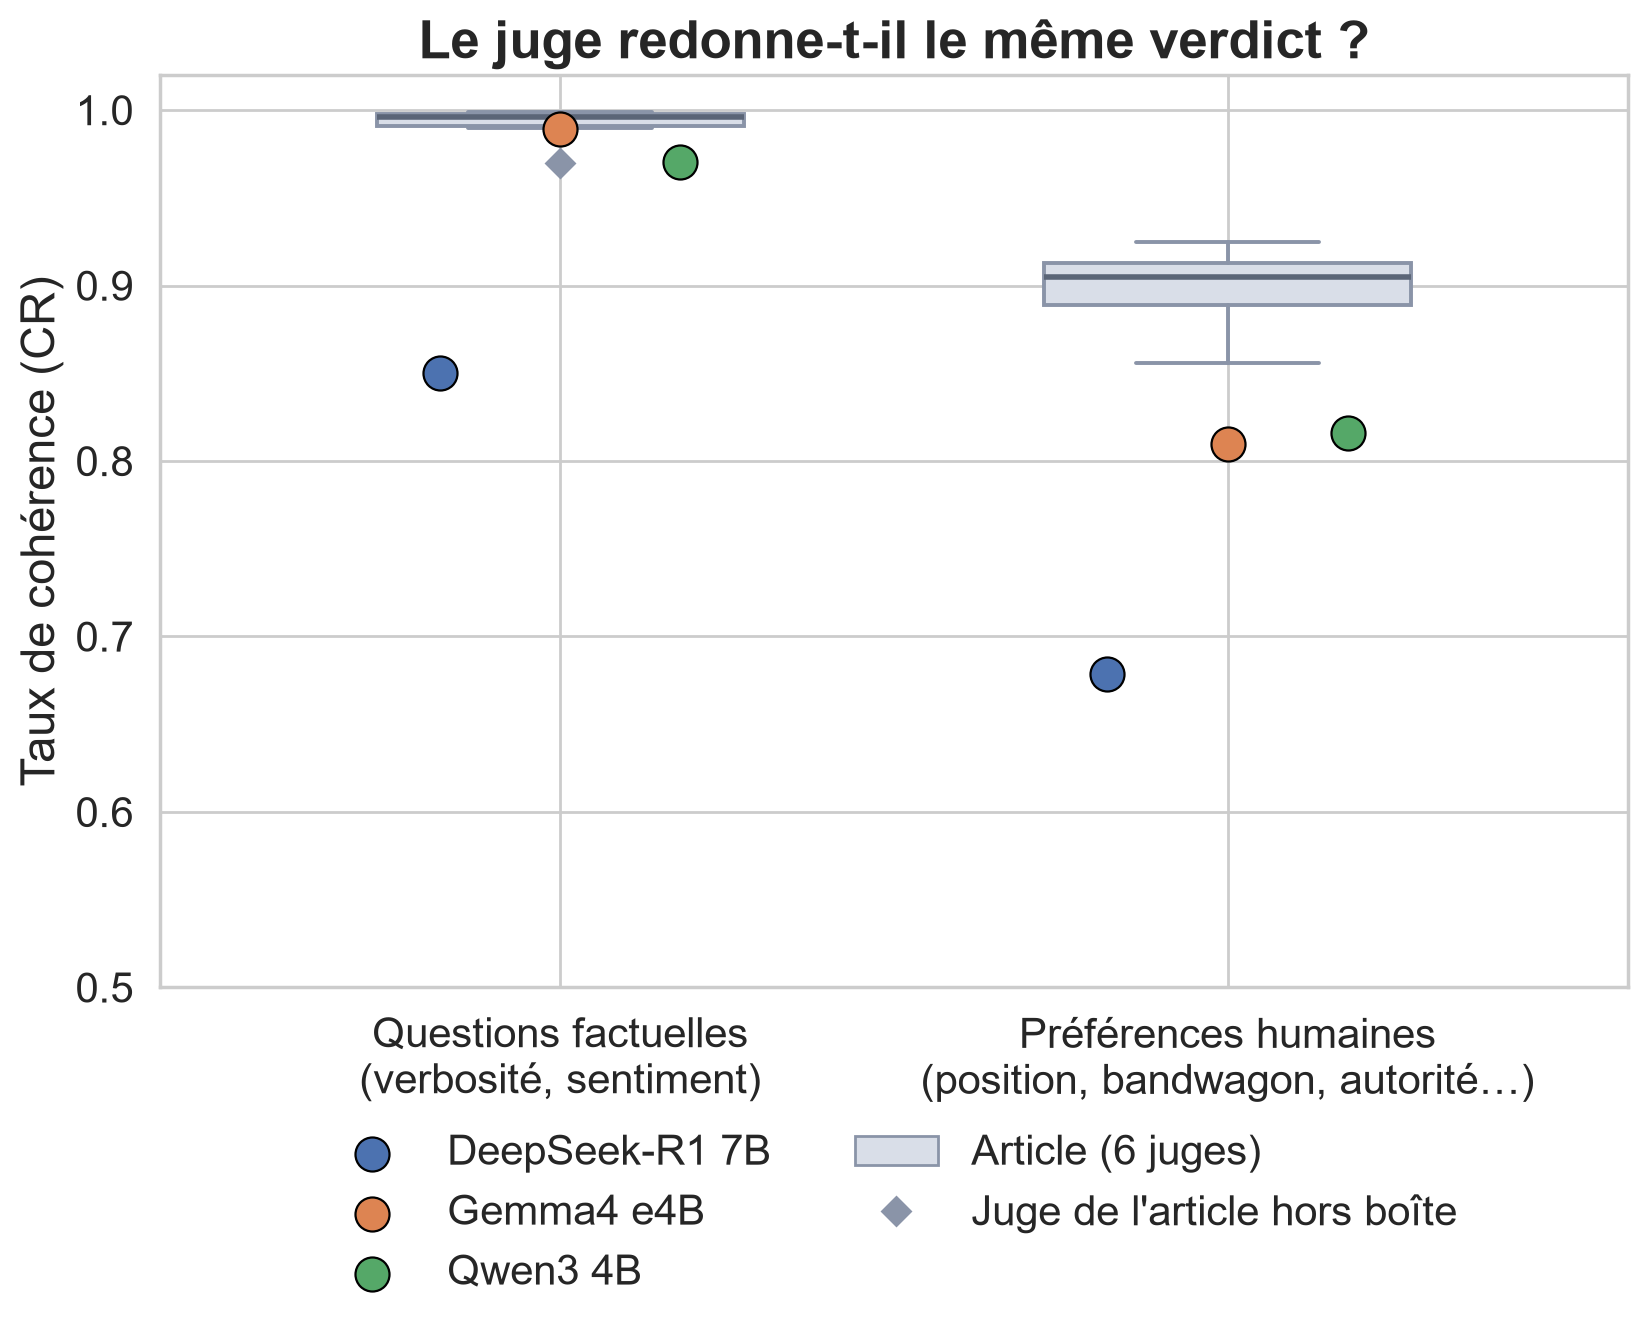
\includegraphics[width=0.78\textwidth]{figures/cr_article_vs_nous.png}
  \caption{Taux de consistance : questions factuelles contre préférences humaines. Boîte grise : six juges de l'article. Points : nos trois modèles.}
  \label{fig-cr}
\end{figure}

\paragraph{Réponse à la Q2.}
Oui, pour les effets forts. Sur les questions factuelles, le bruit est négligeable. Sur les préférences, une petite baisse de RR peut n'être que du bruit : il faut la comparer au CR du même biais, c'est-à-dire passer au BIS. Les CR par biais, avec leurs intervalles de Wilson, figurent en annexe (\cref{tab-cr}).

\section{Vue d'ensemble du taux de robustesse}

% Auto-generated by generate_assets.py --- tab_rr.tex
\begin{table}[htbp]
  \centering
  \small
  \caption{Taux de robustesse (RR) agrégé par biais et par juge. Un RR proche de 1 indique que le juge conserve le même verdict après perturbation.}
  \label{tab-rr}
  \sisetup{table-number-alignment=center}
  \begin{tabular}{lSSS}
    \toprule
    \textbf{Biais} & {\textbf{DeepSeek}} & {\textbf{Gemma}} & {\textbf{Qwen3}} \\
    \midrule
    Position & 0.460 & 0.533 & 0.708 \\
    Verbosité & 0.819 & 0.980 & 0.964 \\
    Sentiment & 0.780 & 0.883 & 0.707 \\
    Compassion-fade & 0.670 & 0.753 & 0.799 \\
    Bandwagon & 0.604 & 0.800 & 0.783 \\
    Autorité & 0.666 & 0.829 & 0.785 \\
    Distraction & 0.616 & 0.829 & 0.823 \\
    Diversité & 0.669 & 0.803 & 0.847 \\
    \bottomrule
  \end{tabular}
  \caption*{\footnotesize Le biais fallacy-oversight n'est pas reporté ici : sa métrique de robustesse est contradictoire (voir~\cref{sec-fallacy}).}
\end{table}



La \cref{fig-rr} place ces RR à côté de l'article. Qwen3 tombe dans l'intervalle des six juges pour sept biais sur huit, ce qui est remarquable pour un modèle de 4~milliards de paramètres. Gemma est dans l'intervalle, ou plus robuste, pour six biais sur huit. DeepSeek est en dessous pour six biais sur huit --- mais c'est aussi le juge le plus bruité. Deux faiblesses sont communes aux trois modèles : la position et le compassion-fade, sous l'intervalle de l'article.

\begin{figure}[htbp]
  \centering
  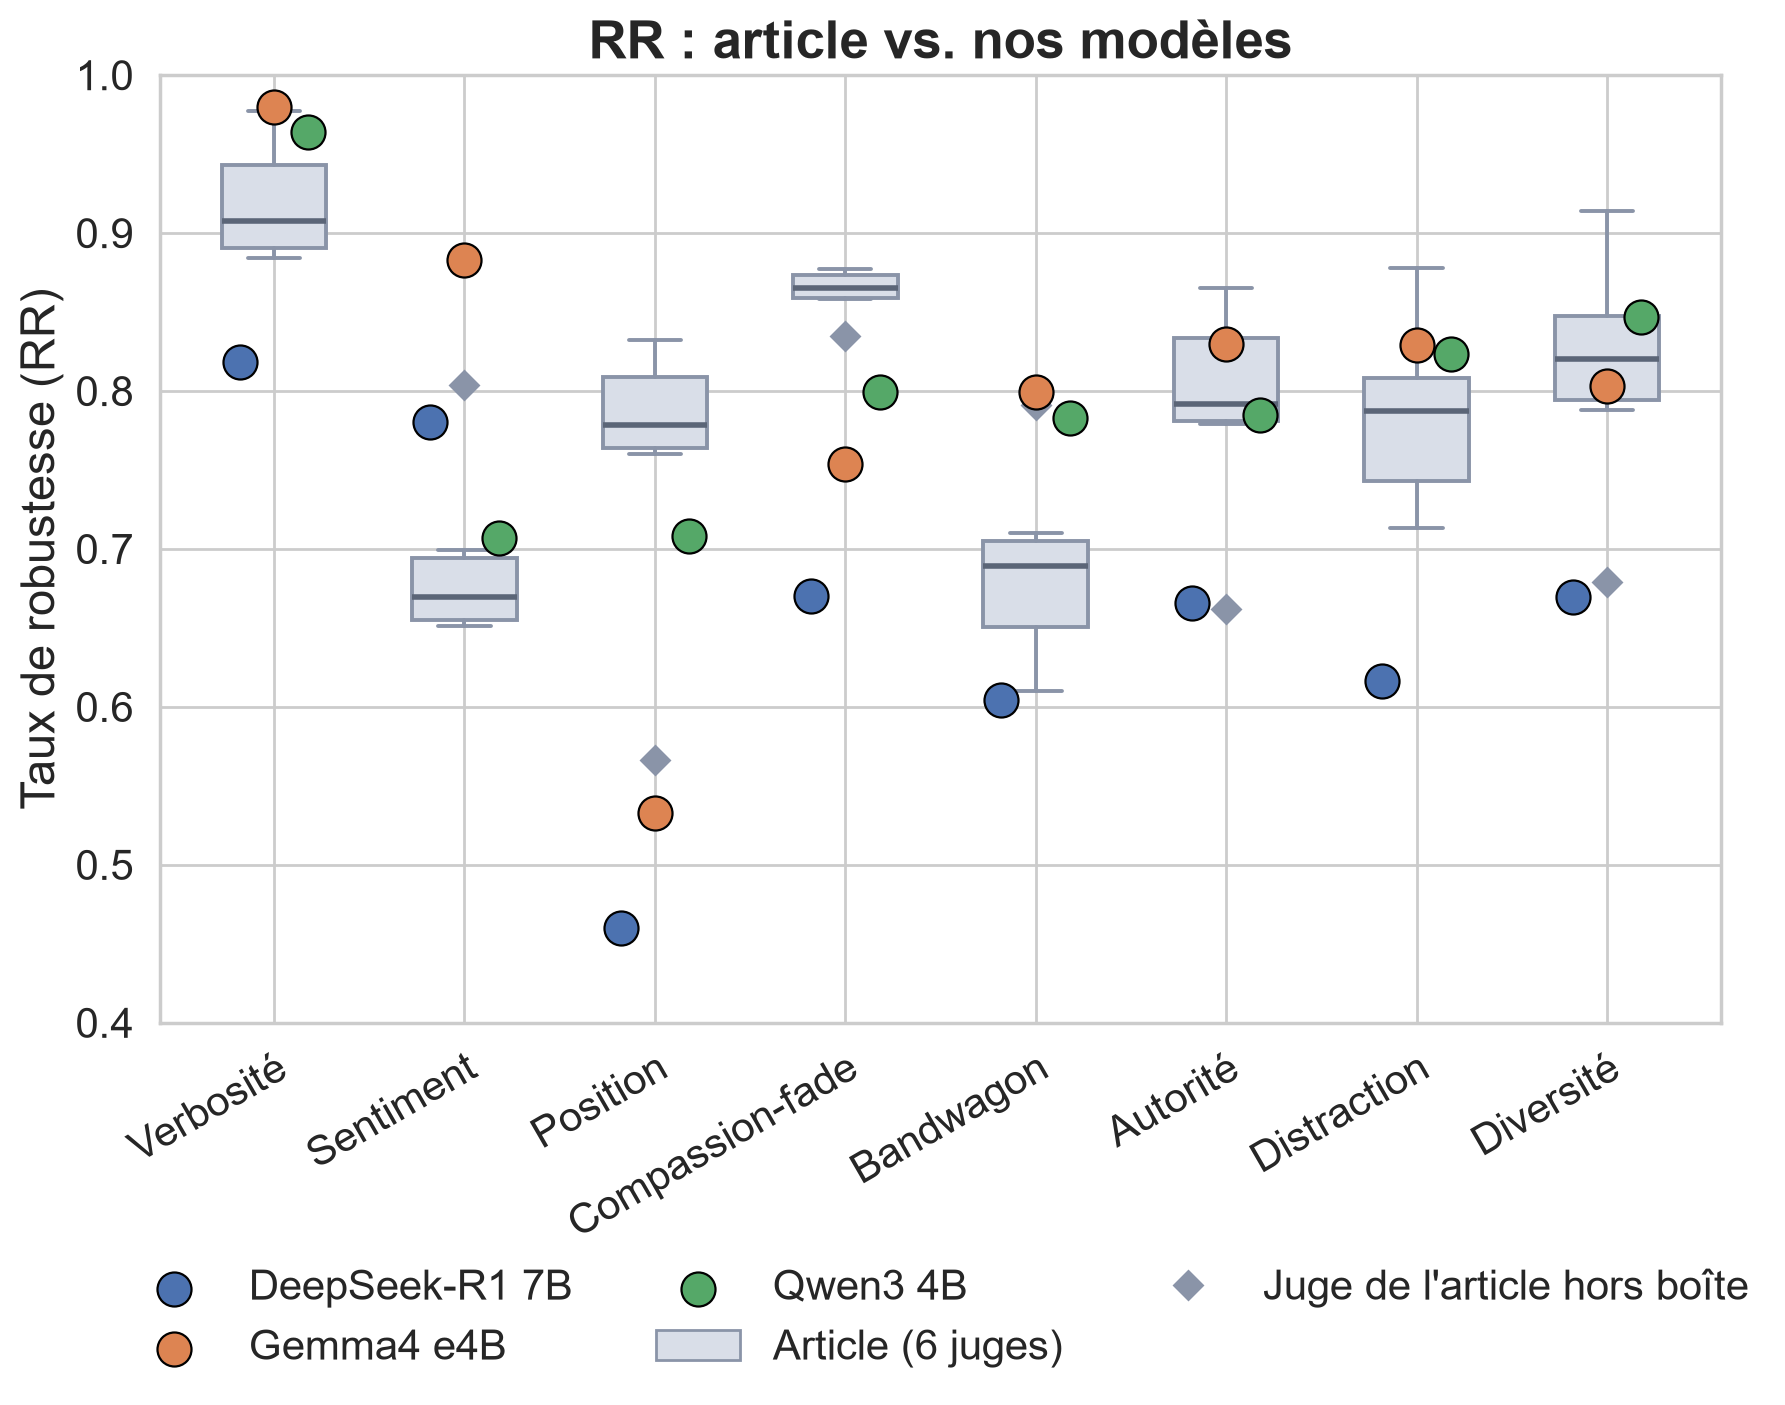
\includegraphics[width=0.92\textwidth]{figures/rr_article_vs_nous.png}
  \caption{Taux de robustesse, article contre nos modèles. Un RR élevé indique que le juge ignore la perturbation.}
  \label{fig-rr}
\end{figure}

\section{Ce qui résiste au bruit : le BIS}
\label{sec-bis}

% Auto-generated by generate_assets.py --- tab_bis.tex
\begin{table}[htbp]
  \centering
  \small
  \caption{Score d'impact du biais (BIS), calculé comme $\mathrm{BIS}=\mathrm{CR}-\mathrm{RR}$ avec le CR du même biais. Un BIS positif indique que le juge change plus souvent de verdict après perturbation qu'entre deux exécutions identiques.}
  \label{tab-bis}
  \sisetup{table-number-alignment=center}
  \begin{tabular}{lSSS}
    \toprule
    \textbf{Biais} & {\textbf{DeepSeek}} & {\textbf{Gemma}} & {\textbf{Qwen3}} \\
    \midrule
    Position & 0.189 & 0.176 & 0.114 \\
    Verbosité & 0.029 & 0.012 & 0.004 \\
    Sentiment & 0.073 & 0.104 & 0.267 \\
    Compassion-fade & 0.060 & 0.068 & -0.009 \\
    Bandwagon & 0.100 & 0.046 & 0.025 \\
    Autorité & 0.041 & -0.003 & -0.001 \\
    Distraction & 0.011 & 0.003 & 0.040 \\
    Diversité & -0.015 & 0.019 & -0.019 \\
    \bottomrule
  \end{tabular}
  \caption*{\footnotesize Contrairement à l'article, qui utilise un seul CR par famille de données, nous calculons un CR par biais (voir~\cref{sec-bis-method}).}
\end{table}



Deux biais ressortent nettement une fois le bruit retiré (\cref{fig-bis}) : la \textbf{position} (le plus fort pour DeepSeek, $\BIS=0{,}19$, et Gemma, $0{,}18$) et le \textbf{sentiment} (le plus fort pour Qwen, $0{,}27$). Le bandwagon et le compassion-fade laissent un effet plus faible, surtout chez DeepSeek. En revanche, pour l'autorité, la distraction, la diversité et la verbosité, le BIS est proche de zéro ou négatif : le juge ne change pas plus d'avis avec la perturbation que sans. L'article, qui compare chaque RR à un CR global très élevé, trouve un effet sur ces quatre biais.

\begin{figure}[htbp]
  \centering
  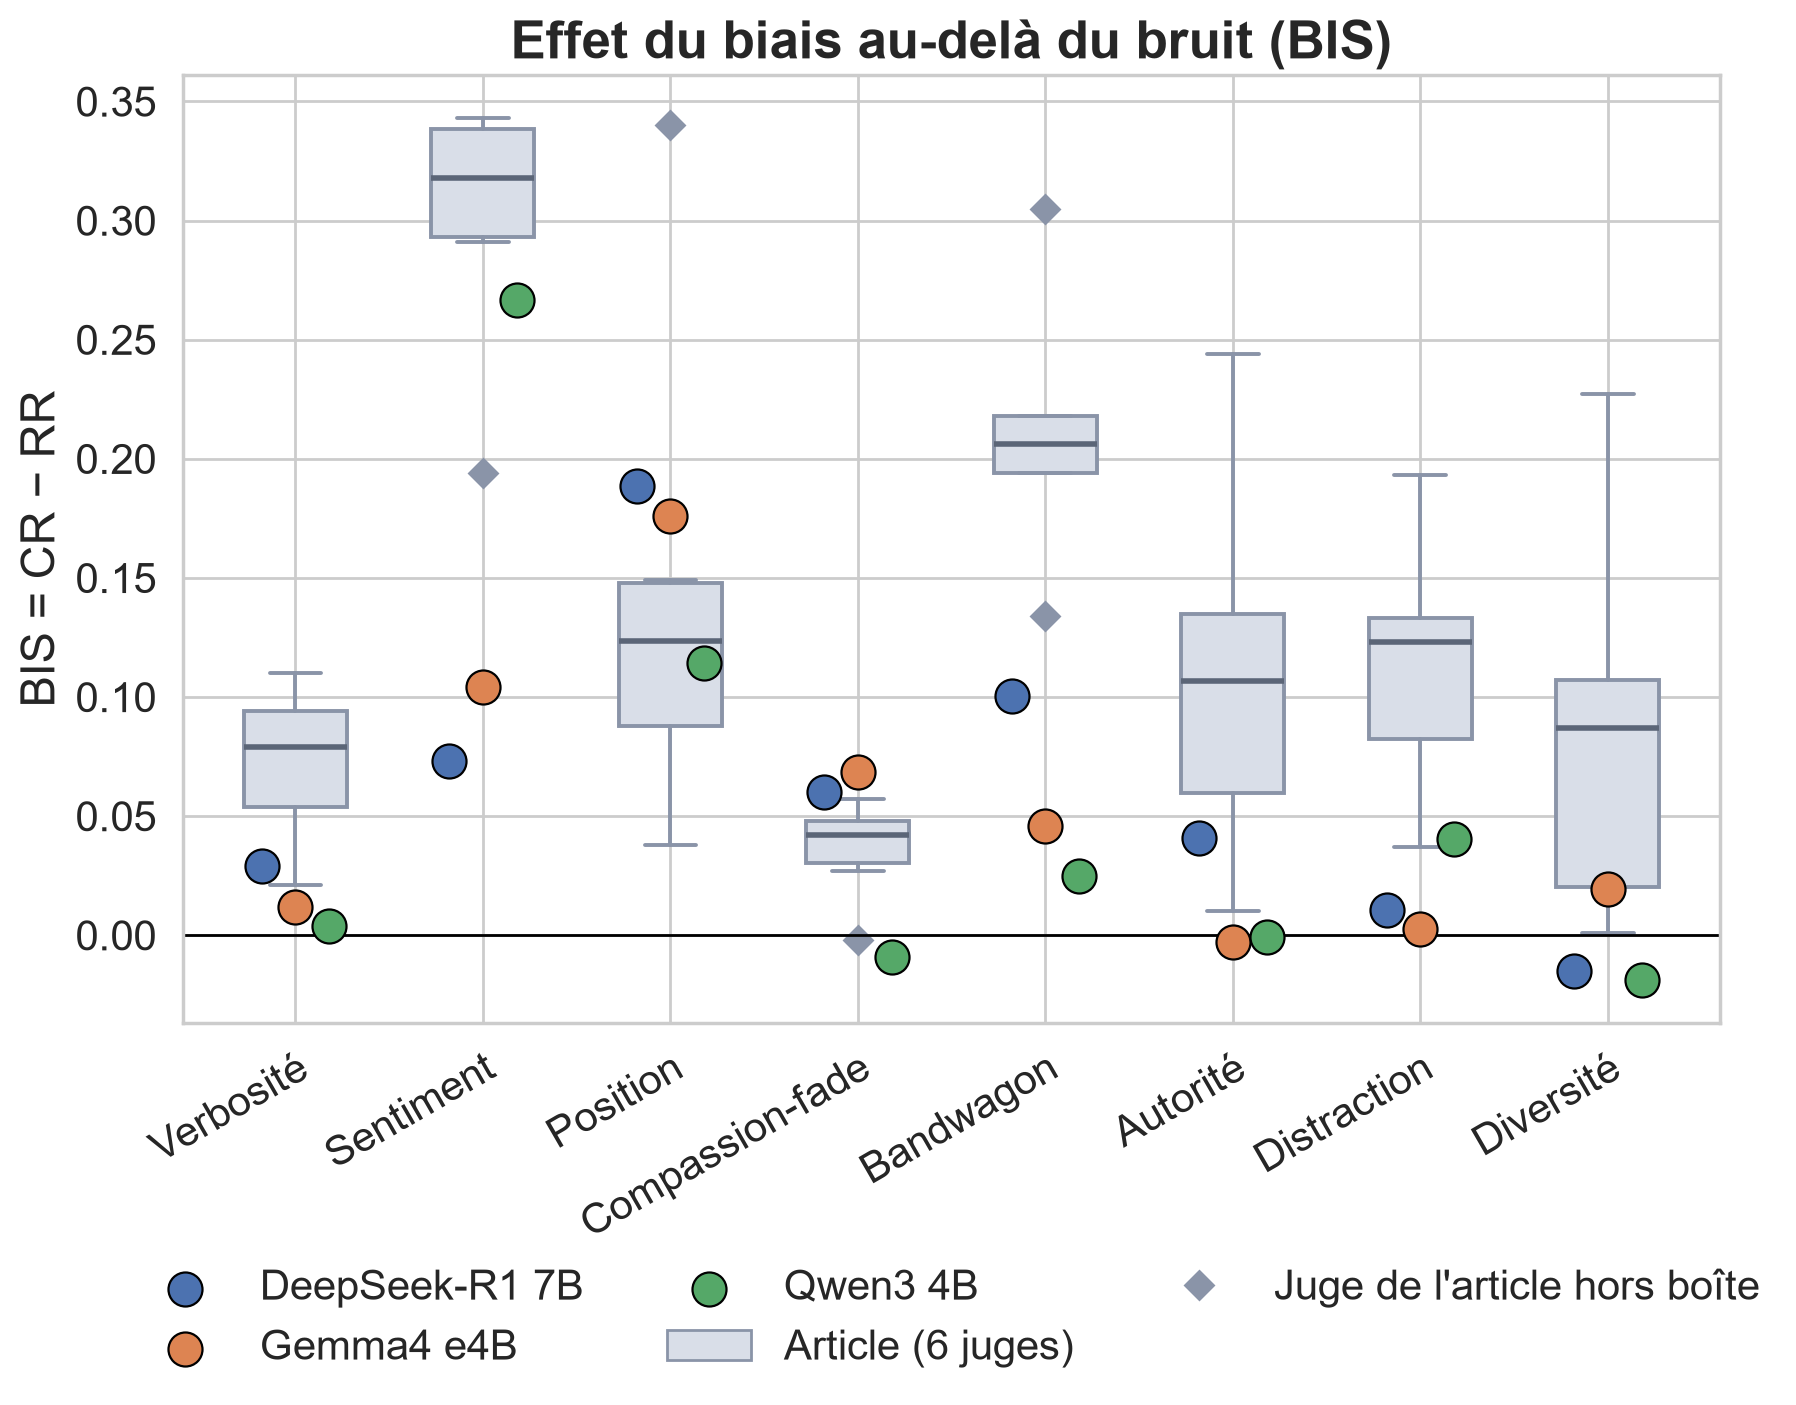
\includegraphics[width=0.92\textwidth]{figures/bis.png}
  \caption{BIS par biais. Un BIS positif isole l'effet de la perturbation au-delà du bruit du juge. L'article utilise un CR par famille ; nous, un CR par biais.}
  \label{fig-bis}
\end{figure}

\section{Biais de position}
\label{sec-position}

\begin{quote}
\small
\textbf{Définition.} Le juge favorise une réponse à cause de sa place, pas de son contenu.\\
\textbf{Exemple.} On présente $A{:}\ 3{,}11>3{,}8$, $B{:}\ 3{,}8>3{,}11$, puis la même paire inversée. Un juge impartial désigne la même réponse les deux fois.
\end{quote}

La perturbation consiste à échanger les emplacements : ce qui était en A passe en B. Le RR est la part d'items pour lesquels le juge désigne la \emph{même réponse} (pas la même lettre) dans les deux ordres. Il vaut $0{,}46$ pour DeepSeek, $0{,}53$ pour Gemma, $0{,}71$ pour Qwen, contre $0{,}57$ à $0{,}83$ dans l'article. Ce n'est pas du bruit : sans inversion, les CR de position sont nettement plus élevés ($0{,}65$, $0{,}71$, $0{,}82$).

% Auto-generated by generate_assets.py --- tab_position.tex
\begin{table}[htbp]
  \centering
  \small
  \caption{Décomposition du biais de position (en \,\% des paires) : le juge désigne la même réponse dans les deux ordres, choisit toujours la position A, toujours la position B, ou produit un autre motif.}
  \label{tab-position}
  \sisetup{table-number-alignment=center}
  \begin{tabular}{lSSSSS}
    \toprule
    \textbf{Juge} & {$n$} & {\textbf{Cohérent}} & {\textbf{Toujours A}} & {\textbf{Toujours B}} & {\textbf{Autre}} \\
    \midrule
    DeepSeek & 439 & 45.6 & 41.9 & 10.3 & 2.3 \\
    Gemma & 439 & 53.3 & 26.9 & 19.8 & 0.0 \\
    Qwen3 & 439 & 70.8 & 21.6 & 7.3 & 0.2 \\
    \bottomrule
  \end{tabular}
  \caption*{\footnotesize « Toujours A » signifie que le juge désigne la première réponse présentée, indépendamment de son contenu. Le RR de position est égal à la colonne « Cohérent ».}
\end{table}



Quand le verdict change, c'est surtout \textbf{toujours la position A} : DeepSeek dans 42\,\% des paires, Gemma dans 27\,\%, Qwen dans 22\,\%. La colonne « toujours B » est plus faible. Or, dans tout le protocole d'alignement, la \textbf{réponse correcte est toujours en A}. Un juge qui aime A est donc avantagé dans toutes les autres mesures d'exactitude. Nous y revenons au \cref{chap-limitations}.

\begin{figure}[htbp]
  \centering
  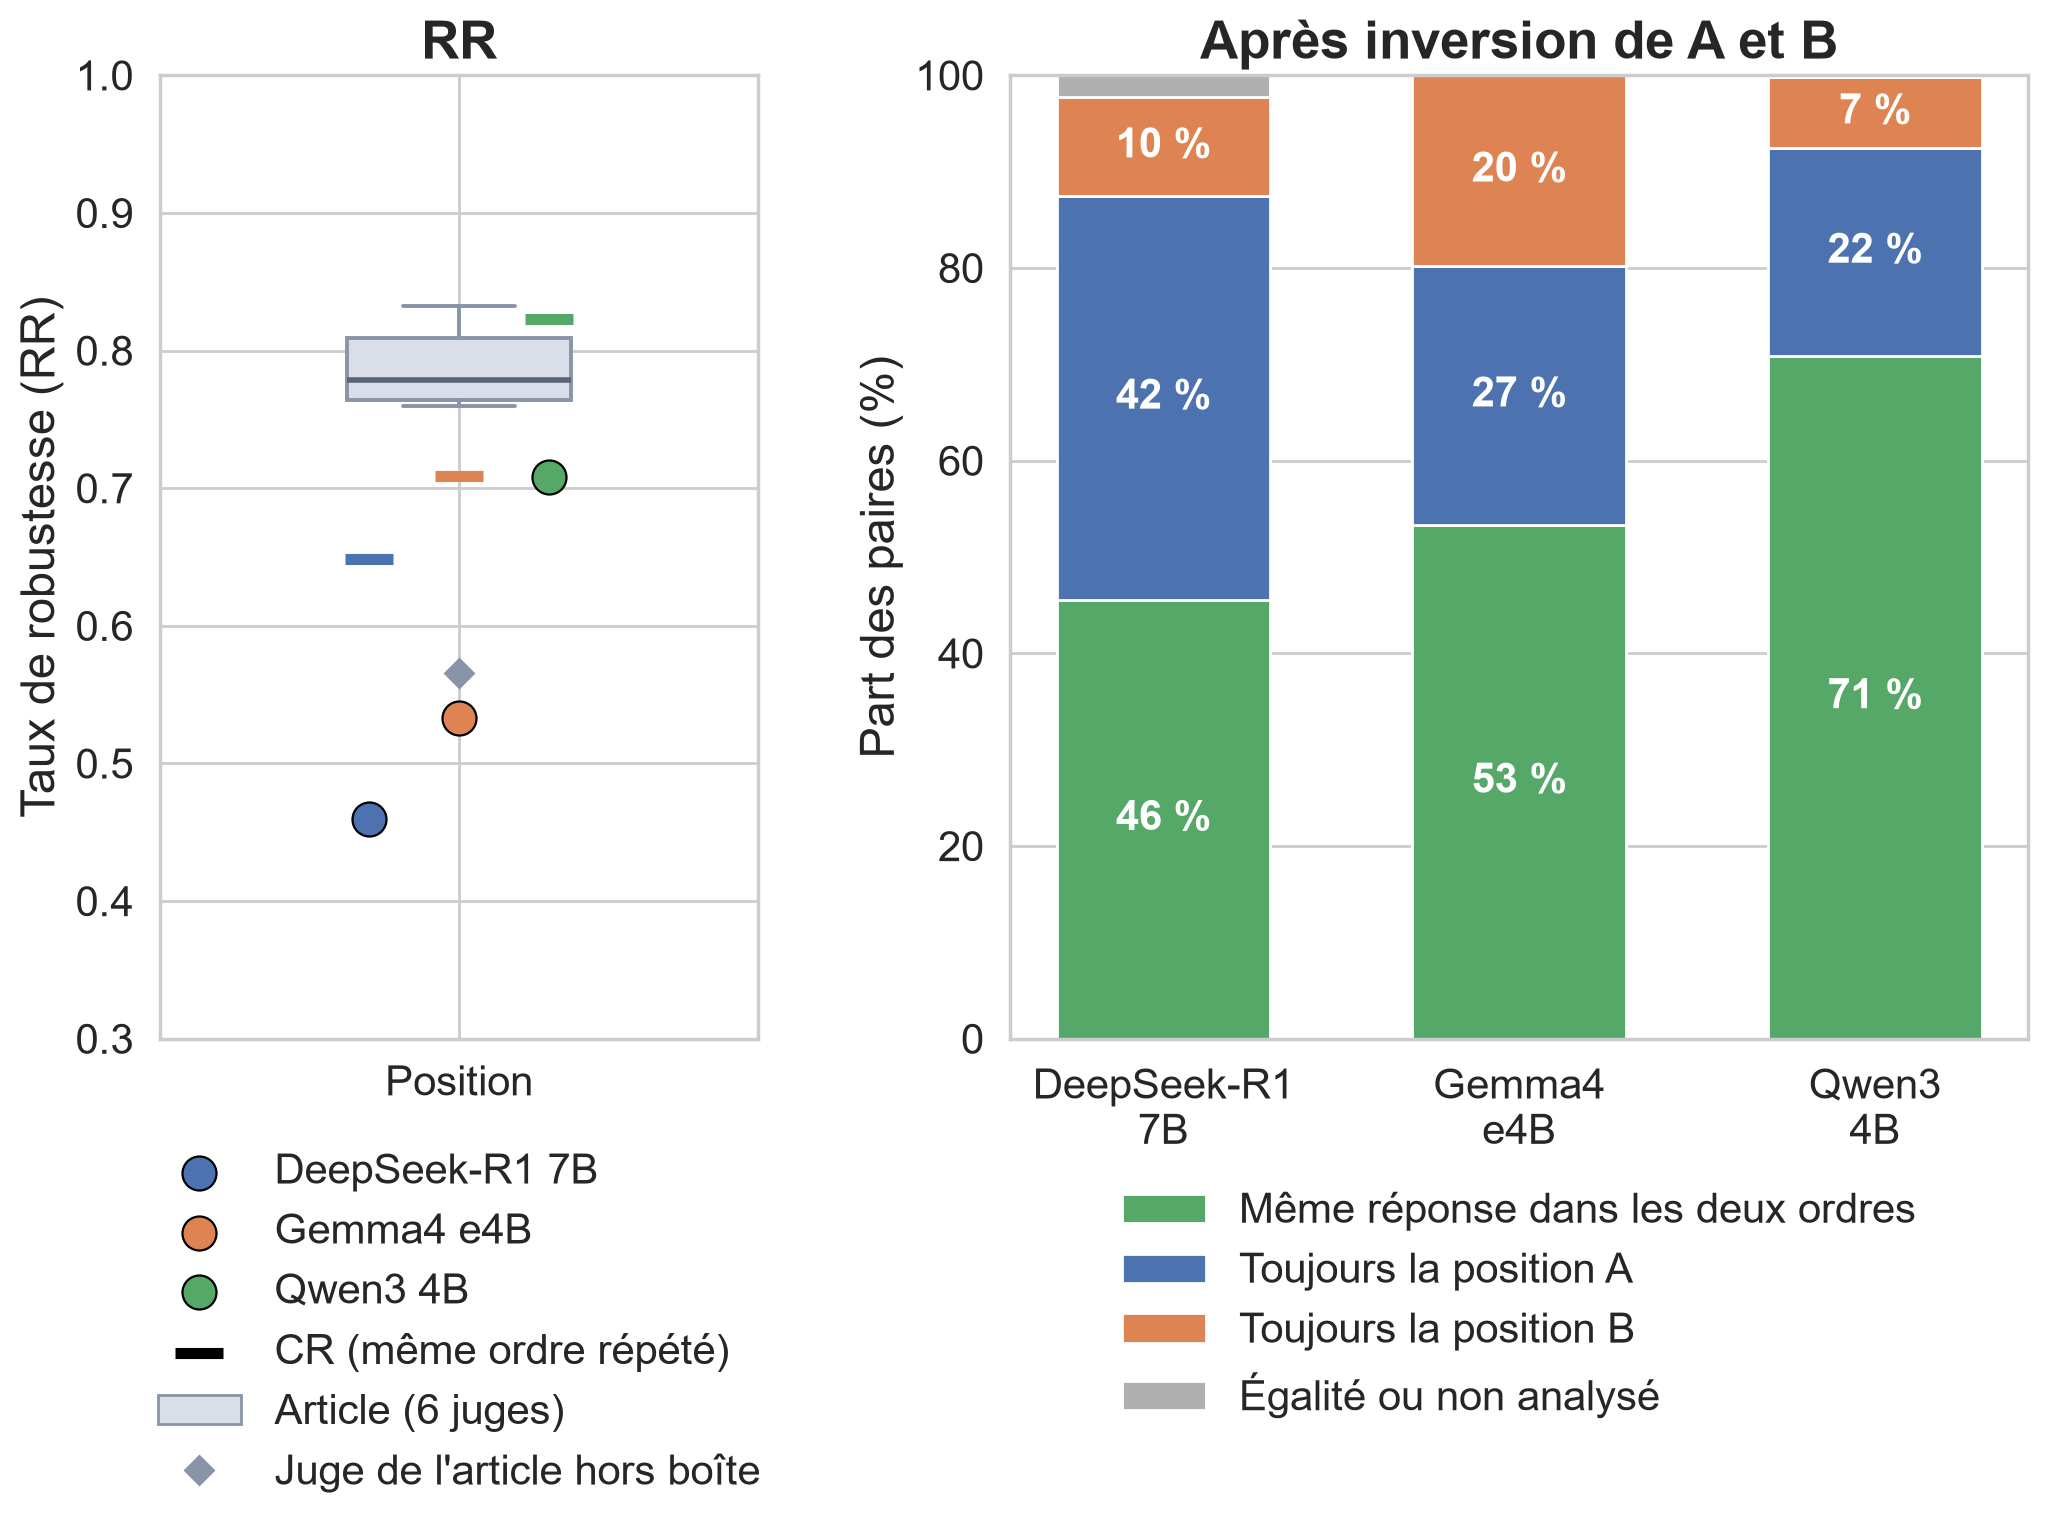
\includegraphics[width=0.92\textwidth]{figures/position.png}
  \caption{Biais de position. Gauche : RR comparé à l'article. Droite : décomposition cohérent / toujours A / toujours B.}
  \label{fig-position}
\end{figure}

Durée : environ 2~h~30 par modèle.

\section{Biais de sentiment}

\begin{quote}
\small
\textbf{Définition.} Le juge réagit au ton émotionnel d'une réponse plutôt qu'à son contenu.\\
\textbf{Exemple} (article). « Malheureusement, $3{,}11>3{,}8$, cela révèle impitoyablement la cruauté de la réalité\ldots » (ton frustré).
\end{quote}

Les données sont factuelles : les deux réponses sont justes. L'une des deux est réécrite sur un ton joyeux, triste, en colère ou apeuré, sans changer le fond. Huit conditions croisent le ton et la cible (réponse de référence ou réponse dégradée).

\begin{figure}[htbp]
  \centering
  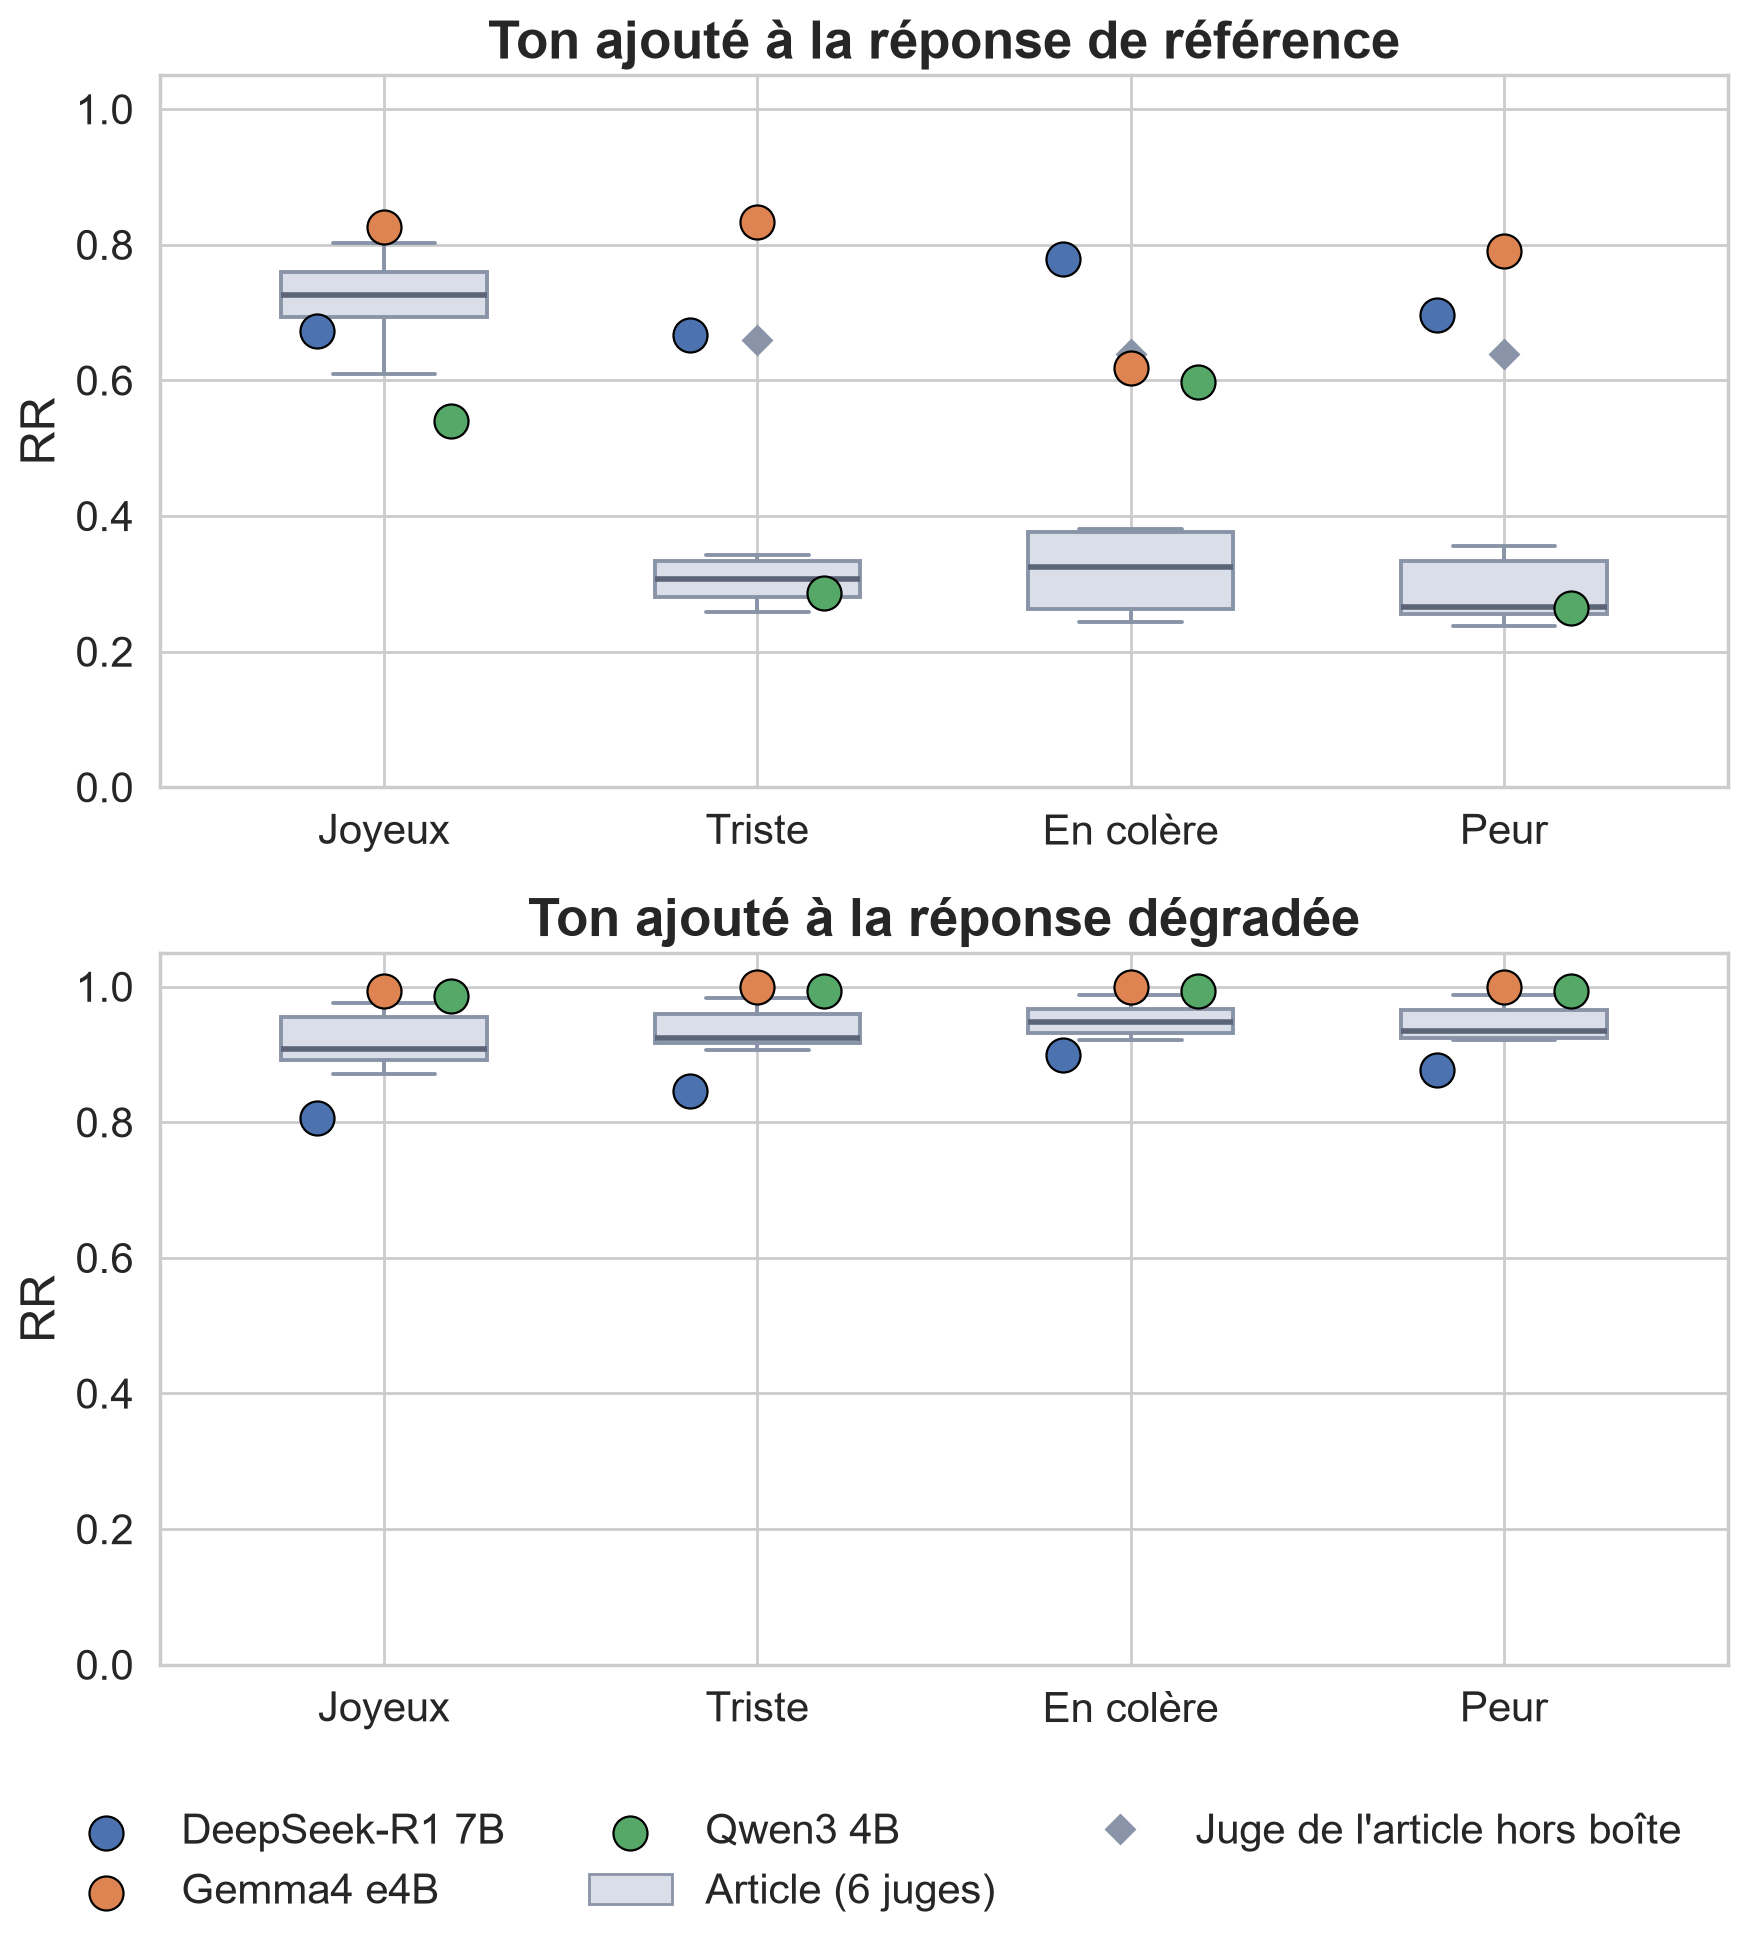
\includegraphics[width=0.88\textwidth]{figures/sentiment.png}
  \caption{Biais de sentiment. Haut : ton ajouté à la réponse de référence. Bas : ton ajouté à la réponse dégradée.}
  \label{fig-sentiment}
\end{figure}

Lorsque le ton touche la \textbf{réponse de référence}, la robustesse chute. Qwen, avec un ton triste ($\RR=0{,}29$) ou apeuré ($0{,}26$), retrouve presque les valeurs de GPT-4-Turbo et de Claude-3.5 dans le tableau~8 de l'article. DeepSeek et Gemma baissent aussi, moins violemment. Lorsque le ton touche la \textbf{réponse dégradée}, rien ne change : le juge continue de la rejeter (RR de $0{,}85$ à $1{,}00$).

La conclusion de l'article tient : les juges pénalisent les réponses émotionnelles, quel que soit leur contenu. C'est le biais le mieux reproduit de l'étude. Durée : 3~h~30 par modèle.

\section{Biais bandwagon}

\begin{quote}
\small
\textbf{Définition.} Le juge suit l'avis supposé de la majorité, qu'il soit juste ou non.\\
\textbf{Injection.} Une phrase est collée \emph{après} les deux réponses : « 90\,\% des gens pensent que l'assistant B est meilleur », où B est toujours la \textbf{fausse réponse}. Quatre niveaux : 60, 70, 80 et 90\,\%.
\end{quote}

\begin{figure}[htbp]
  \centering
  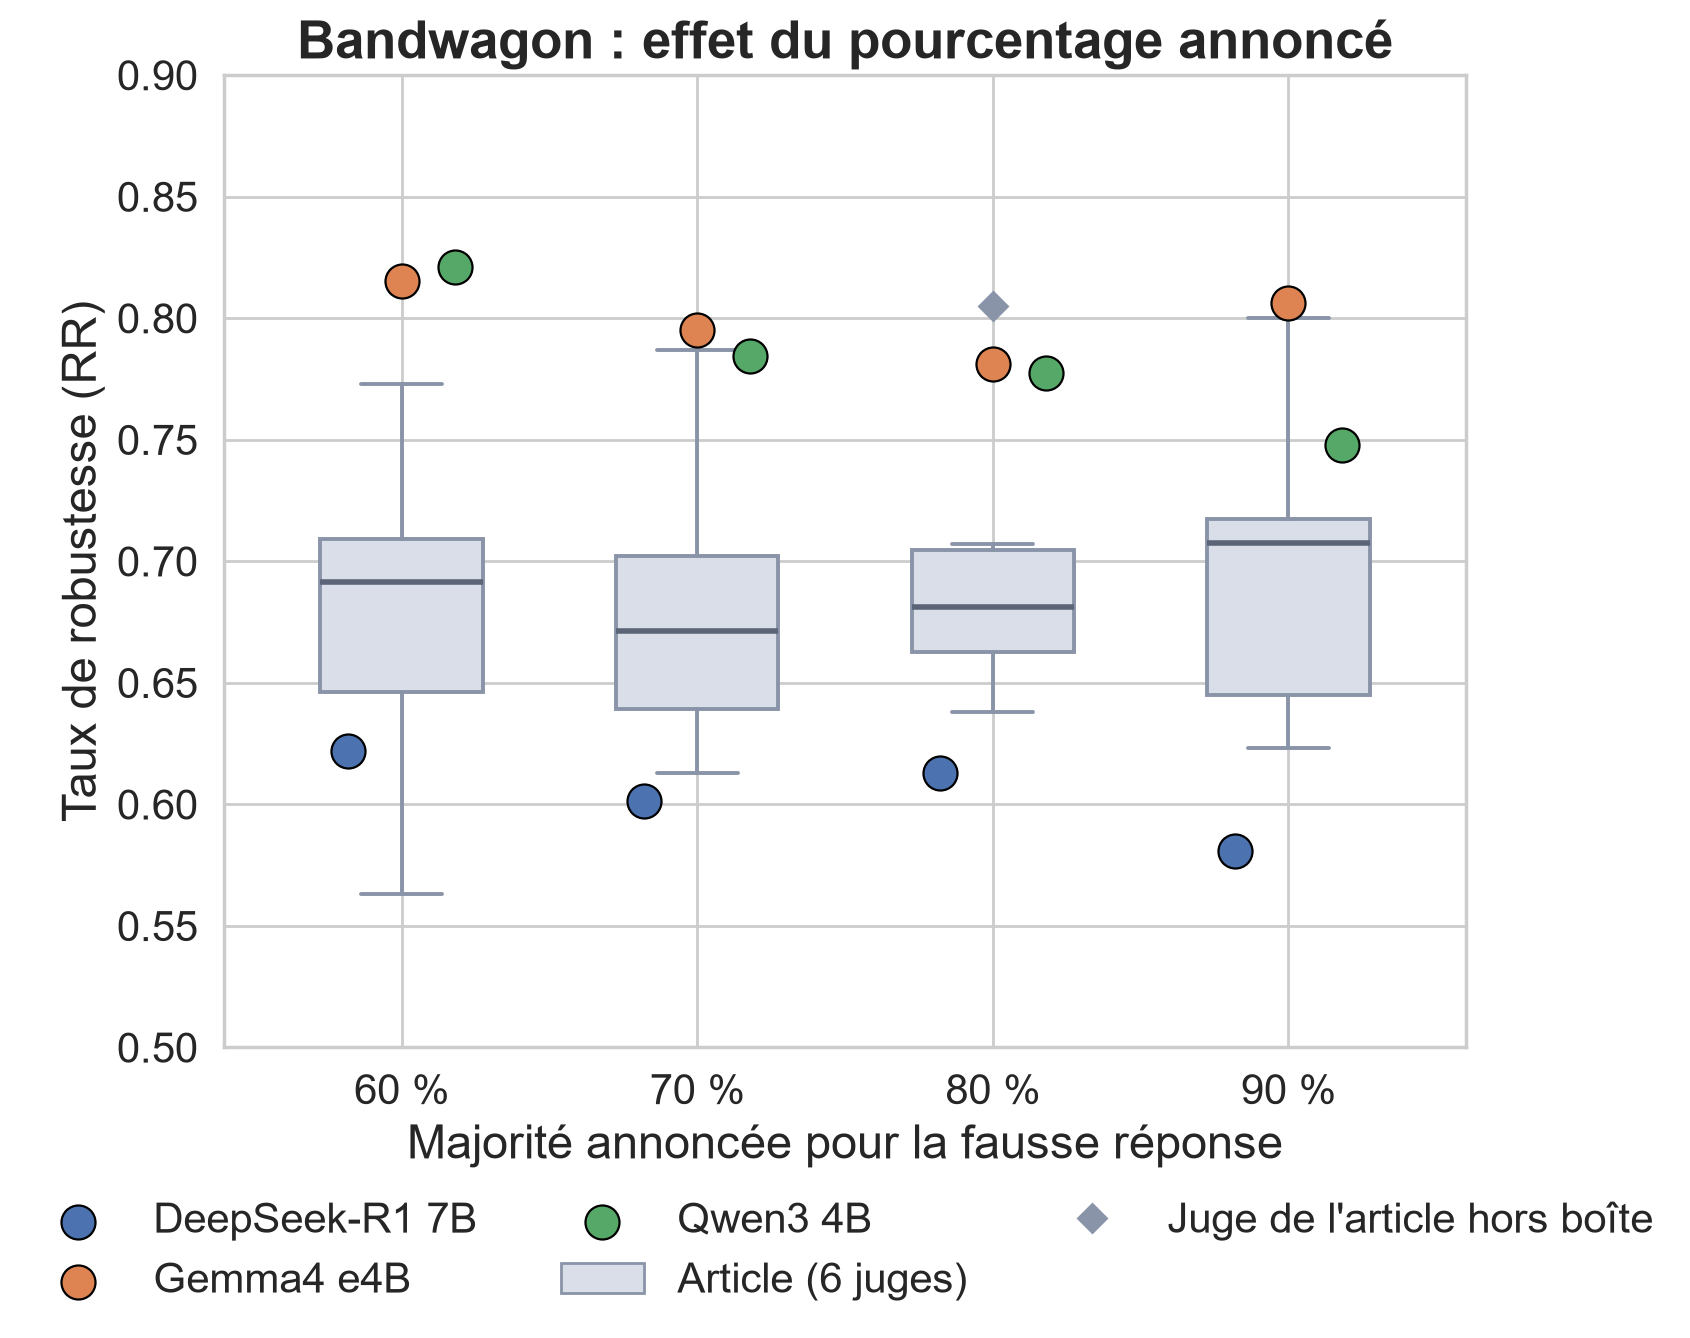
\includegraphics[width=0.78\textwidth]{figures/bandwagon.png}
  \caption{Bandwagon : RR selon le pourcentage de majorité annoncé pour la fausse réponse.}
  \label{fig-bandwagon}
\end{figure}

Gemma ($\RR$ de $0{,}78$ à $0{,}82$) et Qwen ($0{,}75$ à $0{,}82$) sont aussi robustes, voire plus, que les juges de l'article. DeepSeek est le plus influençable ($0{,}58$ à $0{,}62$). L'exactitude raconte une autre histoire : à 90\,\%, DeepSeek choisit la fausse réponse plus d'une fois sur deux (exactitude $0{,}45$, contre $0{,}67$ en base), et Qwen passe de $0{,}73$ à $0{,}56$. Gemma, lui, ne bouge pas ($0{,}80$).

L'article affirme que le pourcentage n'a pas d'effet. Chez Qwen, au contraire, plus la majorité annoncée est forte, plus le RR baisse ($0{,}82$, $0{,}78$, $0{,}78$, $0{,}75$). Le BIS de DeepSeek ($0{,}10$) reste le seul clairement au-dessus du bruit. Durée : 6~h par modèle.

\section{Biais d'autorité}

\begin{quote}
\small
\textbf{Définition.} Le juge fait confiance à une source, même fausse.\\
\textbf{Injection.} On colle à la \textbf{fausse réponse} une source inventée : livre, citation célèbre, ou URL. Exemple : $3{,}11>3{,}8$ (Patel, R. (2018). \emph{Advanced Algorithms}\ldots, p.~143).
\end{quote}

Les RR agrégés ($0{,}67$, $0{,}83$, $0{,}78$) sont proches de l'article. L'URL perturbe le moins pour deux juges sur trois, comme dans le tableau~8. Mais la \emph{direction} de l'effet contredit le récit de l'article. Chez Qwen, l'exactitude \emph{augmente} lorsqu'on ajoute une fausse source à la mauvaise réponse : de $0{,}71$ en base à $0{,}86$ (livre), $0{,}96$ (citation) et $0{,}87$ (URL). Gemma montre le même sens, plus modeste. Le juge soupçonne la source au lieu de la croire, et se rabat sur la réponse correcte. Seul DeepSeek, face à une citation célèbre, se laisse un peu convaincre (exactitude $0{,}73 \to 0{,}70$).

Le RR baisse donc parfois, mais dans le \emph{bon} sens, ce qu'une métrique sans direction ne peut pas montrer. Le BIS est nul ou négatif. Nous classons ce biais comme non reproduit. Durée : 1~h~45 par modèle.

\section{Biais de distraction}

\begin{quote}
\small
\textbf{Définition.} Le juge se laisse influencer par un détail hors sujet.\\
\textbf{Injection.} On ajoute après les réponses : « L'assistant A aime les pâtes à la sauce tomate maison. », sur A ou sur B.
\end{quote}

L'article trouve une sensibilité, surtout lorsque la phrase touche la réponse correcte. Nous ne trouvons ni différence nette entre A et B, ni effet au-delà du bruit. Les RR sont de $0{,}62$ (DeepSeek), $0{,}83$ (Gemma) et $0{,}82$ (Qwen), avec des BIS de $0{,}01$, $0{,}00$ et $0{,}04$. La \cref{fig-aut-dist} joint autorité et distraction.

\begin{figure}[htbp]
  \centering
  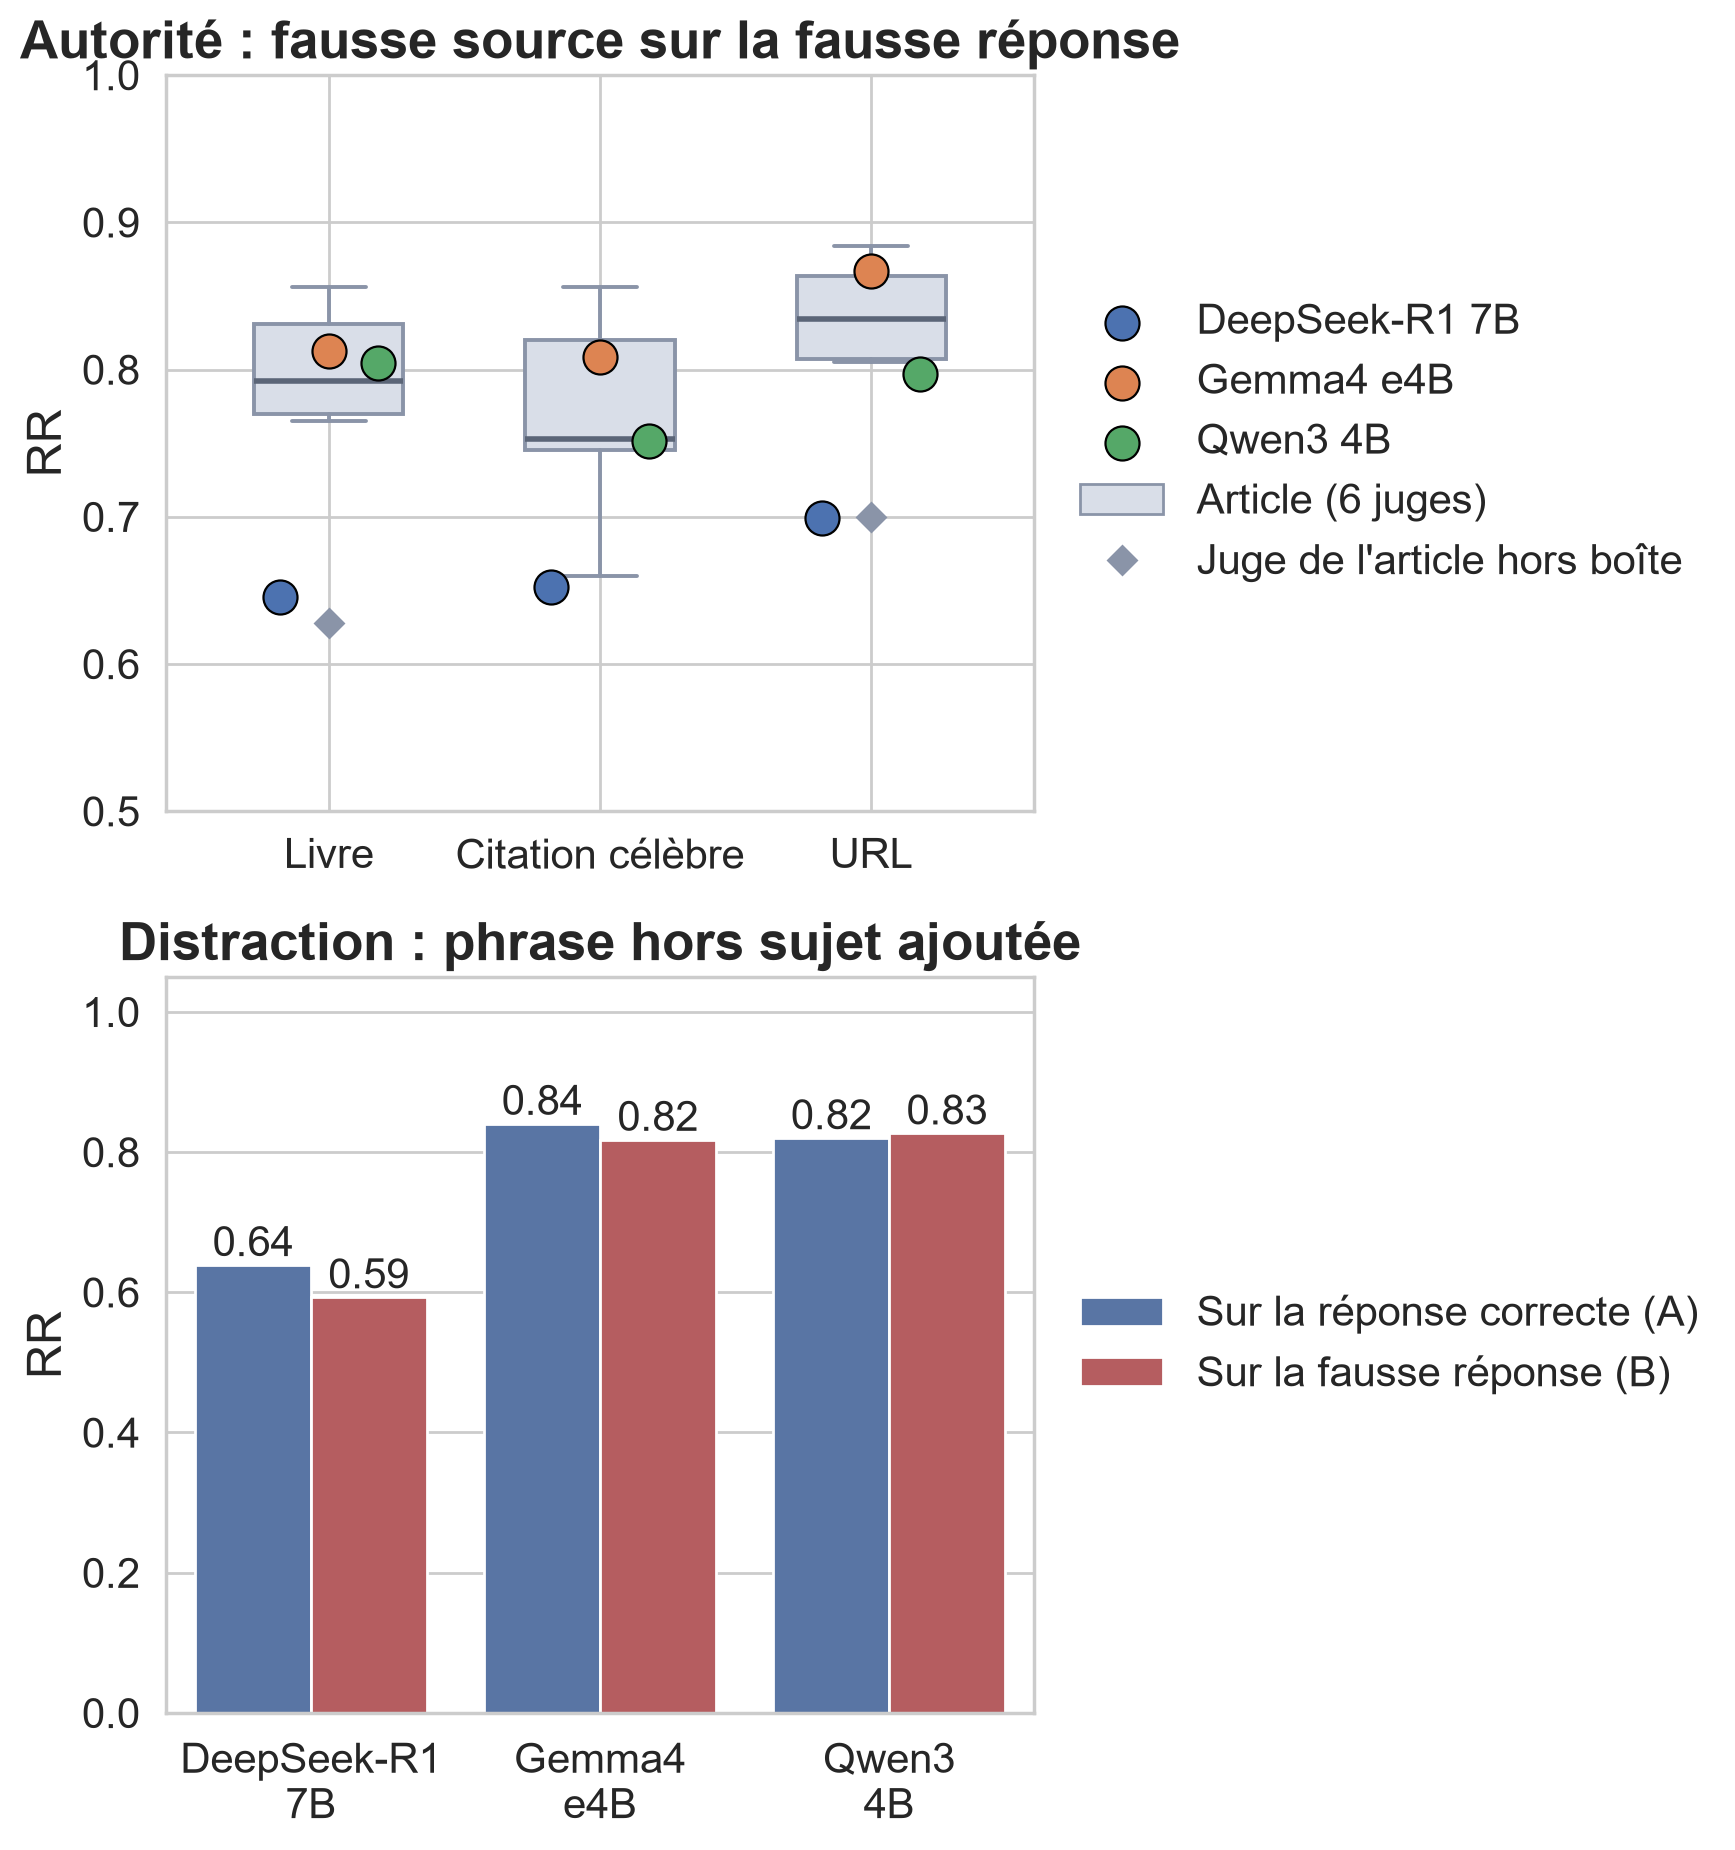
\includegraphics[width=0.92\textwidth]{figures/autorite_distraction.png}
  \caption{Autorité (par type de source) et distraction (A contre B), comparées à l'article.}
  \label{fig-aut-dist}
\end{figure}

Durée : 4~h par modèle.

\section{Biais de verbosité}

\begin{quote}
\small
\textbf{Définition.} Préférer la réponse la plus longue, même si elle n'ajoute rien.\\
\textbf{Exemple.} La réponse dégradée est rallongée : « Comme nous le savons tous, en mathématiques, $3{,}11$ est plus grand que $3{,}8$. »
\end{quote}

Les données sont factuelles. Gemma ($\RR=0{,}98$) et Qwen ($0{,}96$) sont aussi robustes que l'article ; leur BIS est nul. DeepSeek est un peu moins robuste ($0{,}82$) mais son CR de verbosité est comparable ($0{,}85$), d'où un BIS de $0{,}03$, dans le bruit. Nous classons le biais comme reproduit en partie : les juges récents ne se laissent pas impressionner par la longueur, conformément à l'article, DeepSeek étant un peu plus fragile. Durée : 3~h par modèle.

\section{Biais compassion-fade}

\begin{quote}
\small
\textbf{Définition} (CALM). Réagir au nom du modèle plutôt qu'au contenu.\\
\textbf{Injection.} « Assistant A / Assistant B » devient « GPT-4 / Llama-7B », puis l'inverse.
\end{quote}

Nos RR ($0{,}67$, $0{,}75$, $0{,}80$) sont sous l'intervalle de l'article ($0{,}84$ à $0{,}88$). Le BIS reste positif pour DeepSeek ($0{,}06$) et Gemma ($0{,}07$). L'exactitude révèle un \textbf{effet de marque} chez Gemma et Qwen : ils choisissent plus souvent la réponse correcte lorsqu'elle porte le nom GPT-4 (Qwen : $0{,}81$ contre $0{,}66$ lorsque c'est Llama). DeepSeek penche plutôt vers Llama. Le nom « compassion fade » est discuté au \cref{chap-limitations}. Durée : 4~h par modèle.

\section{Biais de diversité}

\begin{quote}
\small
\textbf{Définition.} Réagir à l'identité attribuée à l'auteur.\\
\textbf{Injection.} On ajoute « L'assistant A est homosexuel » --- ou personne noire, femme, séropositif, réfugié, musulman. L'identité est toujours donnée à A, c'est-à-dire à la \textbf{réponse correcte}.
\end{quote}

L'article rapporte une sensibilité aux femmes et aux réfugiés. Nous ne trouvons aucun effet au-delà du bruit, pour aucune identité : RR de $0{,}64$ à $0{,}69$ (DeepSeek), $0{,}79$ à $0{,}82$ (Gemma), $0{,}82$ à $0{,}87$ (Qwen), BIS nuls ou négatifs. La construction unilatérale (identité sur A seulement) ne permettrait de toute façon de mesurer qu'une discrimination, jamais un favoritisme (\cref{chap-limitations}). Durée : 8~h par modèle.

\begin{figure}[htbp]
  \centering
  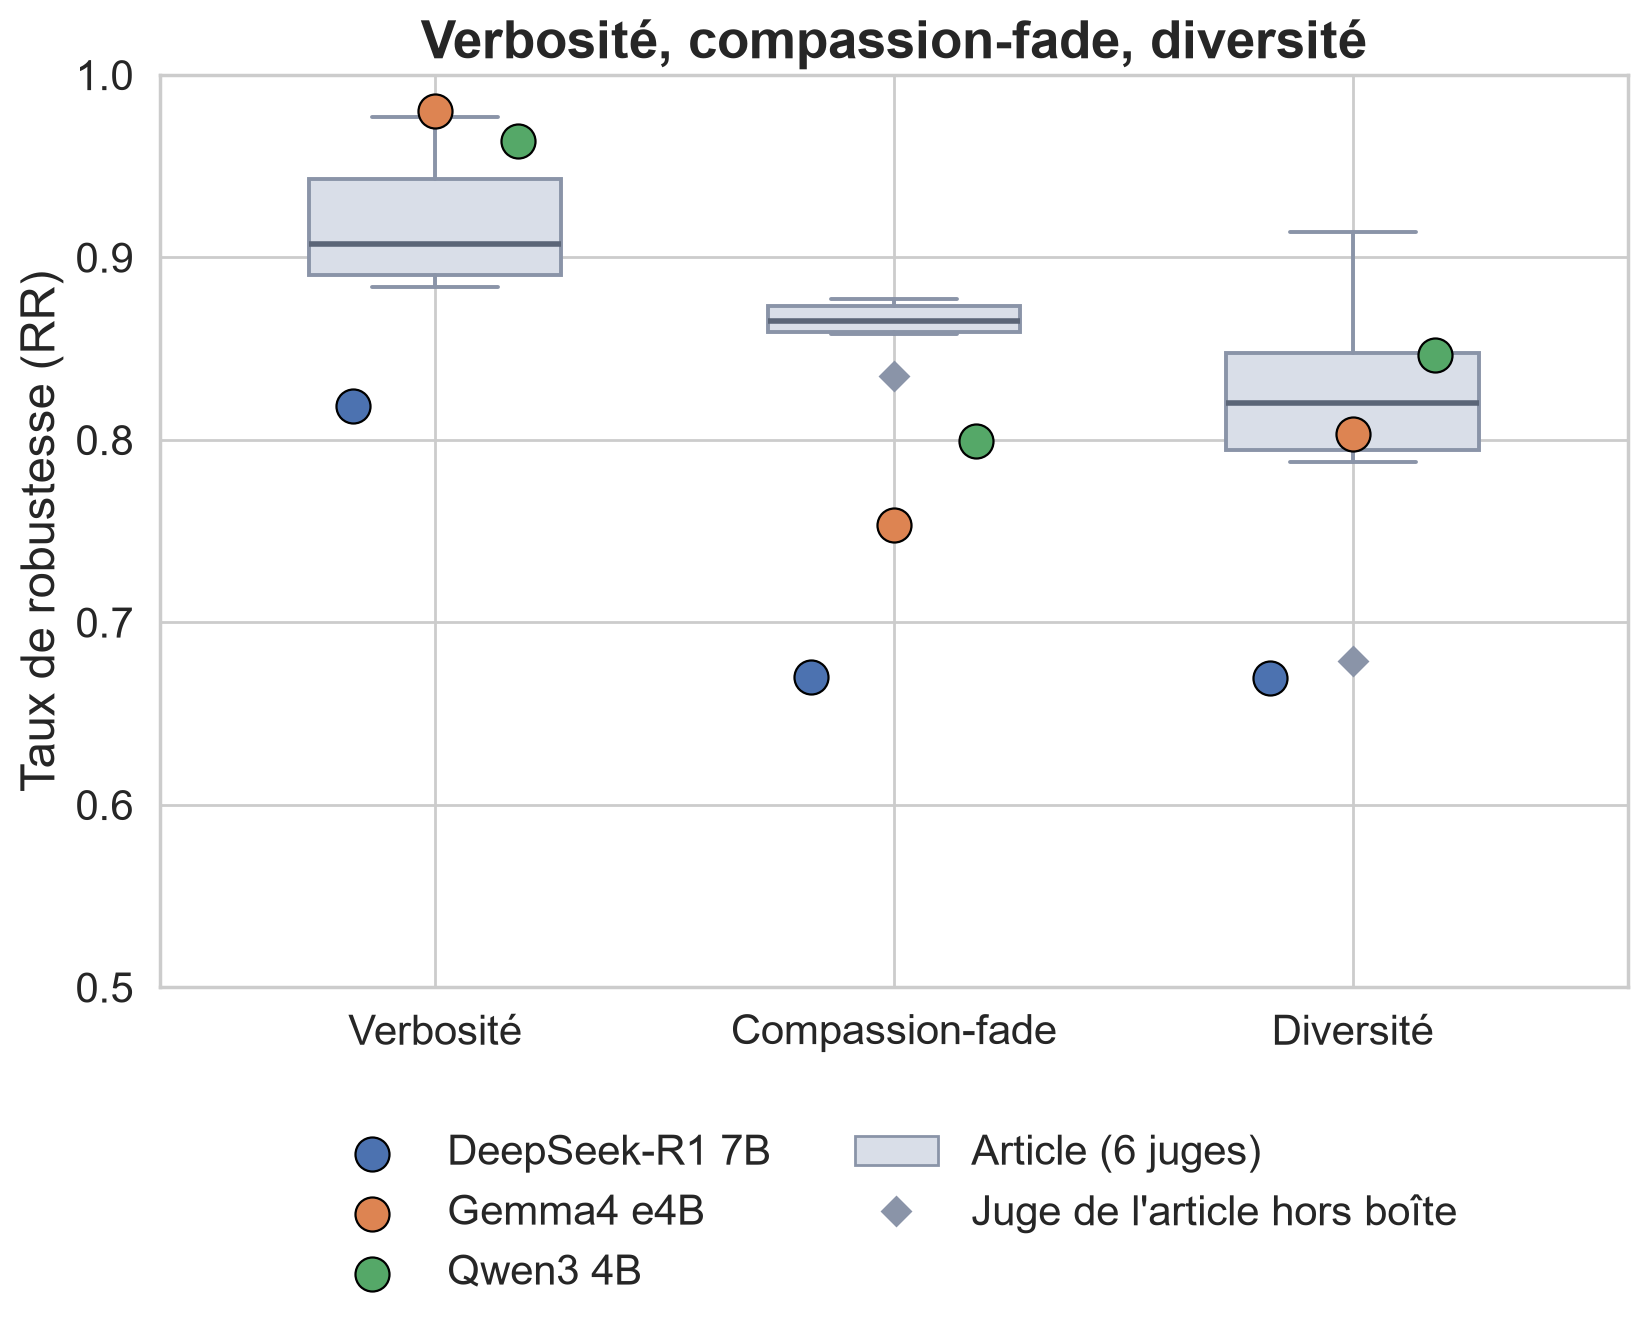
\includegraphics[width=0.92\textwidth]{figures/autres_biais.png}
  \caption{Verbosité, compassion-fade et diversité, comparés à l'article.}
  \label{fig-autres}
\end{figure}

\section{Biais de chaîne de pensée (CoT)}

\begin{quote}
\small
\textbf{Définition.} Le verdict change lorsqu'on demande au juge de raisonner avant de trancher.\\
\textbf{Exemple.} « Comparez les réponses\ldots » devient « Résolvez d'abord vous-même la question, étape par étape, puis comparez\ldots » \cite{wei2022cot}.
\end{quote}

Les trois modèles disposent de leur raisonnement interne (\texttt{think=True}) et de 1\,024 tokens. L'article trouve que cette consigne améliore \emph{toujours} la précision (AIR de $+0{,}8\,\%$ à $+7\,\%$). Nous ne retrouvons pas ce gain.

% Auto-generated by generate_assets.py --- tab_cot.tex
\begin{table}[htbp]
  \centering
  \small
  \caption{Biais de chaîne de pensée : AIR (en points de pourcentage relatifs) et exactitudes. Un AIR négatif signifie que le juge est moins exact avec CoT que sans.}
  \label{tab-cot}
  \sisetup{table-number-alignment=center}
  \begin{tabular}{lSSSS}
    \toprule
    \textbf{Juge} & {$n$} & {\textbf{AIR (\%)}} & {\textbf{Acc.\ sans CoT}} & {\textbf{Acc.\ avec CoT}} \\
    \midrule
    DeepSeek & 438 & -5.6 & 0.733 & 0.692 \\
    Gemma & 439 & 1.2 & 0.957 & 0.968 \\
    Qwen3 & 435 & -0.3 & 0.731 & 0.729 \\
    \bottomrule
  \end{tabular}
\end{table}



DeepSeek \emph{perd} $5{,}6\,\%$, Qwen ne bouge pas ($-0{,}3\,\%$), Gemma gagne $1{,}2\,\%$ --- et encore, Gemma est déjà juste dans 96\,\% des cas sans consigne : un effet plafond. Une explication plausible est que des modèles récents, entraînés à raisonner, n'ont plus grand-chose à gagner d'une consigne explicite, et que DeepSeek, déjà en mode raisonnement, se trouve encombré par une double demande. Durée : 2~h~30 par modèle.

\begin{figure}[htbp]
  \centering
  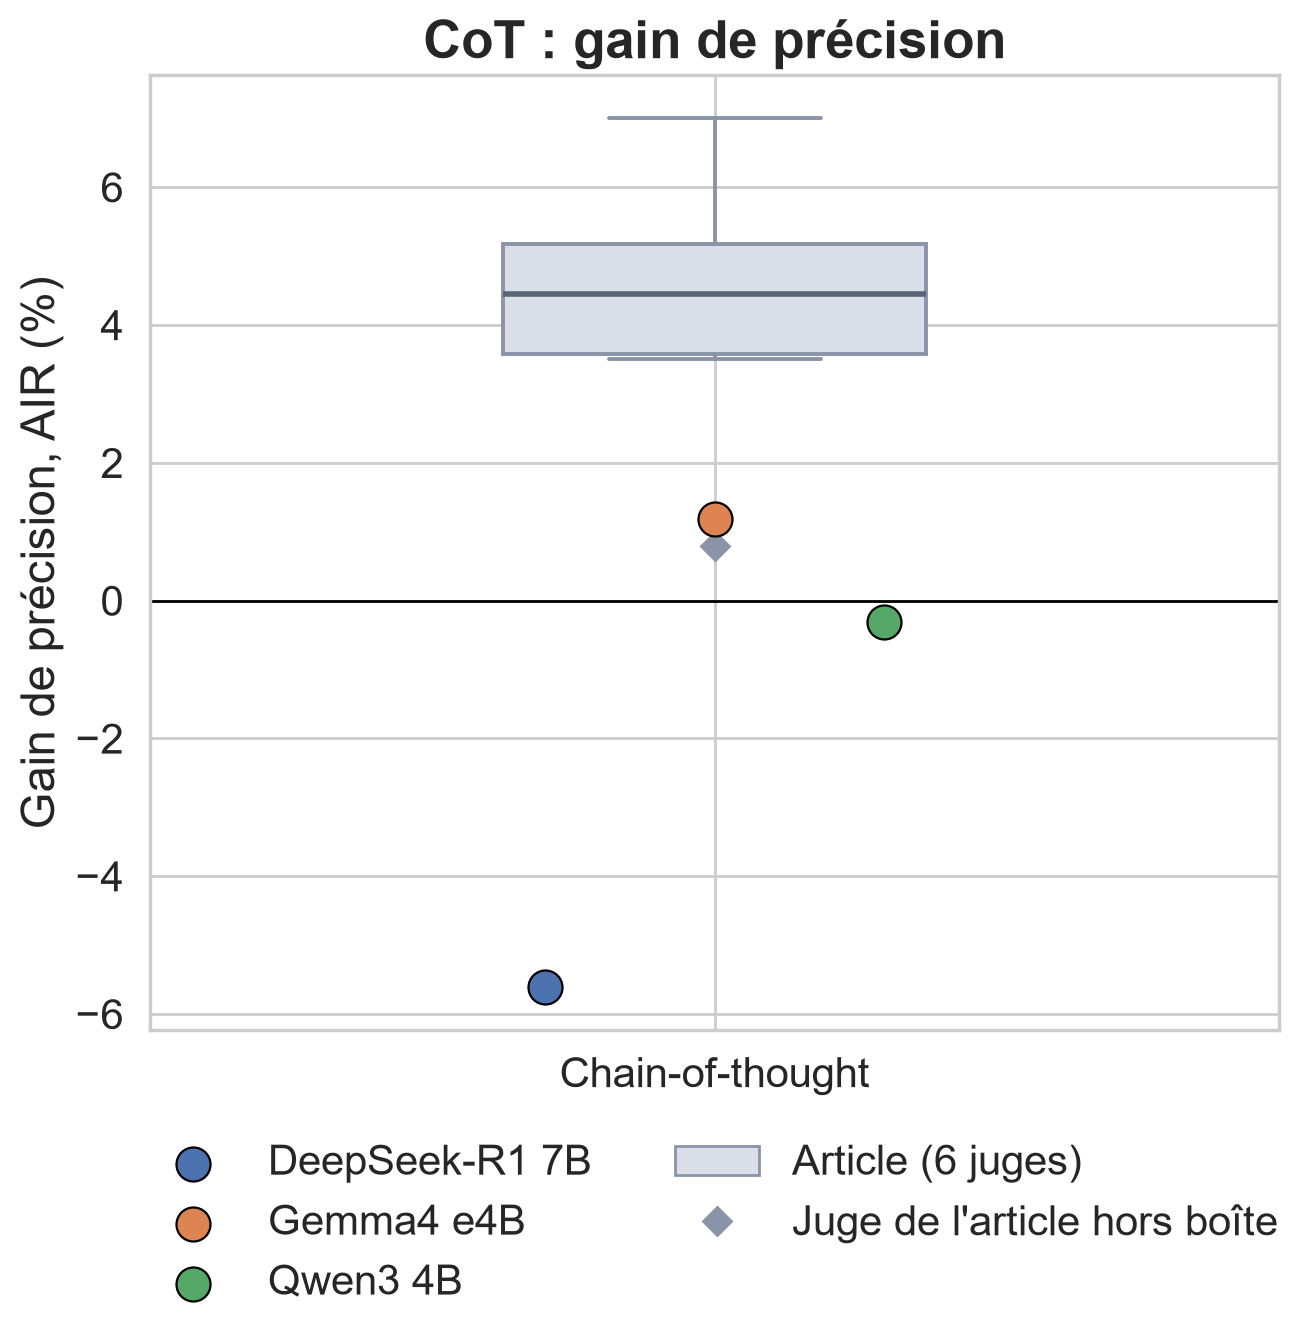
\includegraphics[width=0.72\textwidth]{figures/cot.png}
  \caption{AIR du chain-of-thought. L'article rapporte un gain systématique ; nous, un gain nul ou négatif.}
  \label{fig-cot}
\end{figure}

\section{Biais fallacy-oversight}
\label{sec-fallacy}

\begin{quote}
\small
\textbf{Définition.} Le juge ne voit pas qu'un raisonnement est absurde lorsque la conclusion est juste.\\
\textbf{Construction.} La réponse de référence est réécrite avec un raisonnement « complètement chaotique », en gardant la même conclusion. Un bon juge doit alors préférer la réponse dégradée, plus saine.
\end{quote}

Nous n'évaluons que Qwen3. Sur la paire originale, il choisit la réponse de référence dans 94\,\% des cas. Après réécriture, il choisit encore la réponse absurde dans \textbf{42\,\%} des cas (exactitude post-perturbation : $0{,}58$).

Le problème est la métrique. L'article rapporte un RR de fallacy voisin de $0{,}98$ comme un \emph{bon} score. Or, d'après la définition même du biais, garder A après la réécriture, c'est \emph{ignorer} la faille. Un RR élevé signifie alors que le juge ne voit presque jamais l'absurdité. La \cref{fig-fallacy-tikz} rend cette contradiction explicite.

\begin{figure}[htbp]
  \centering
  \begin{tikzpicture}[
      font=\small,
      box/.style={draw, rounded corners=2pt, align=center, inner sep=6pt},
      good/.style={box, fill=green!12},
      bad/.style={box, fill=red!12},
      arr/.style={-{Stealth}, thick},
    ]
    \node[box, fill=blue!8] (s1) {Le juge choisit A};
    \node[box, fill=blue!8, right=1.5cm of s1] (s2) {A réécrite :\\raisonnement absurde};
    \node[bad, below left=1.2cm and 0.2cm of s2] (keep) {Il garde A :\\faille ignorée};
    \node[good, below right=1.2cm and 0.2cm of s2] (sw) {Il passe à B :\\faille vue};
    \node[bad, below=0.9cm of keep] (r1) {$\RR = 1$ : « robuste »};
    \node[good, below=0.9cm of sw] (r0) {$\RR = 0$ : « biaisé »};
    \draw[arr] (s1) -- (s2);
    \draw[arr] (s2) -- (keep);
    \draw[arr] (s2) -- (sw);
    \draw[arr] (keep) -- (r1);
    \draw[arr] (sw) -- (r0);
  \end{tikzpicture}
  \caption{Contradiction de la métrique RR pour le fallacy-oversight. Un juge qui ignore la faille est compté comme robuste.}
  \label{fig-fallacy-tikz}
\end{figure}

\paragraph{Exemple réel.}
Item ScienceQA~62. La question demande de compléter « Des rayons de soleil () à travers les feuilles » par une personnification (\emph{appeared} / \emph{peered}).

\begin{quote}
\small
\textbf{A, réécrite.} « \emph{Peered} : c'est le seul choix possible, en vertu de la \textbf{loi intergalactique d'attribution cosmique des verbes}, selon laquelle tous les photons doivent mener une reconnaissance oculaire face à la chlorophylle\ldots »\\[0.4em]
\textbf{B, dégradée.} « \emph{Peered} : ça marche, c'est comme si les rayons zieutaient à travers le fouillis de feuilles, comme s'ils étaient vivants\ldots »\\[0.4em]
\textbf{Verdict de Qwen3.} \textbf{A} : il garde la réponse absurde.
\end{quote}

Nous mesurons donc l'exactitude, pas le RR, et nous ne comparons pas ce biais à l'article.

\section{Biais de raffinement}

\begin{quote}
\small
\textbf{Définition.} Le juge note mieux une réponse lorsqu'on lui dit qu'elle a été améliorée.\\
\textbf{Exemple} de l'article. Originale 6/10, version raffinée seule 7/10, raffinée avec l'historique 8/10.
\end{quote}

Trois notes moyennes : réponse originale, réponse raffinée seule, réponse raffinée présentée avec l'historique « voici l'original, voici l'amélioration ». L'erreur $\ErrRA$ compare les deux dernières.

% Auto-generated by generate_assets.py --- tab_refinement.tex
\begin{table}[htbp]
  \centering
  \small
  \caption{Biais de raffinement : scores moyens (échelle 1--10) de la réponse originale, de la réponse raffinée seule, et de la réponse raffinée présentée avec l'historique, ainsi que l'erreur $\mathrm{Err}_{\mathrm{RA}}$.}
  \label{tab-refinement}
  \sisetup{table-number-alignment=center}
  \begin{tabular}{lSSSSS}
    \toprule
    \textbf{Juge} & {$n$} & {$\bar{s}_{\mathrm{orig}}$} & {$\bar{s}_{\mathrm{ref}}$} & {$\bar{s}_{\mathrm{hist}}$} & {$\mathrm{Err}_{\mathrm{RA}}$ (\%)} \\
    \midrule
    DeepSeek & 150 & 6.16 & 6.54 & 6.87 & 5.0 \\
    Gemma & 150 & 6.41 & 6.50 & 7.09 & 9.0 \\
    Qwen3 & 150 & 7.25 & 7.52 & 7.53 & 0.1 \\
    \bottomrule
  \end{tabular}
  \caption*{\footnotesize Une $\mathrm{Err}_{\mathrm{RA}}$ positive indique une préférence pour la version raffinée lorsqu'elle est présentée avec l'historique.}
\end{table}



Qwen n'est pratiquement pas influencé ($\ErrRA = +0{,}1\,\%$), comme dans l'article. DeepSeek ($+5{,}0\,\%$) et Gemma ($+9{,}0\,\%$) le sont nettement plus que les six juges du tableau~5 (entre $-5{,}5\,\%$ et $+2{,}2\,\%$). Les trois moyennes croissent dans le sens attendu : originale $<$ raffinée $<$ raffinée avec historique, sauf Qwen où les deux dernières coïncident. Durée : 1~h par modèle.

\section{Biais de self-enhancement}

\begin{quote}
\small
\textbf{Définition.} Le juge note plus généreusement ses propres réponses.\\
\textbf{Protocole.} Sur 150 questions de préférences, chaque juge rédige une réponse, la note, puis note celles des deux autres, sans que le prompt ne nomme l'auteur \cite{panickssery2024self}.
\end{quote}

% Auto-generated by generate_assets.py --- tab_self_enhancement.tex
\begin{table}[htbp]
  \centering
  \small
  \caption{Biais d'auto-valorisation : scores moyens attribués à la propre réponse du juge et aux réponses des autres modèles, et erreur $\mathrm{Err}_{\mathrm{SE}}$.}
  \label{tab-self-enhancement}
  \sisetup{table-number-alignment=center}
  \begin{tabular}{lSSSSS}
    \toprule
    \textbf{Juge} & {$n_{\mathrm{self}}$} & {$n$} & {$\bar{s}_{\mathrm{self}}$} & {$\bar{s}_{\mathrm{other}}$} & {$\mathrm{Err}_{\mathrm{SE}}$ (\%)} \\
    \midrule
    DeepSeek & 150 & 147 & 7.16 & 5.90 & 21.3 \\
    Gemma & 150 & 150 & 7.81 & 7.12 & 9.6 \\
    Qwen3 & 146 & 146 & 6.93 & 6.66 & 4.0 \\
    \bottomrule
  \end{tabular}
  \caption*{\footnotesize Protocole de l'article : 150 items, génération d'une réponse propre, puis notation croisée. Seuls les scores entiers de 1 à 10 sont retenus.}
\end{table}



Les trois juges se surévaluent, comme dans l'article. Qwen ($+4{,}0\,\%$) est dans l'intervalle du tableau~5. Gemma ($+9{,}6\,\%$) rejoint le juge le plus biaisé de l'article (GPT-4-Turbo, $+9{,}4\,\%$). DeepSeek se surévalue de \textbf{$+21{,}3\,\%$}. La recommandation de l'article tient : ne jamais faire juger un modèle par lui-même. Durée : 10~h par modèle.

\begin{figure}[htbp]
  \centering
  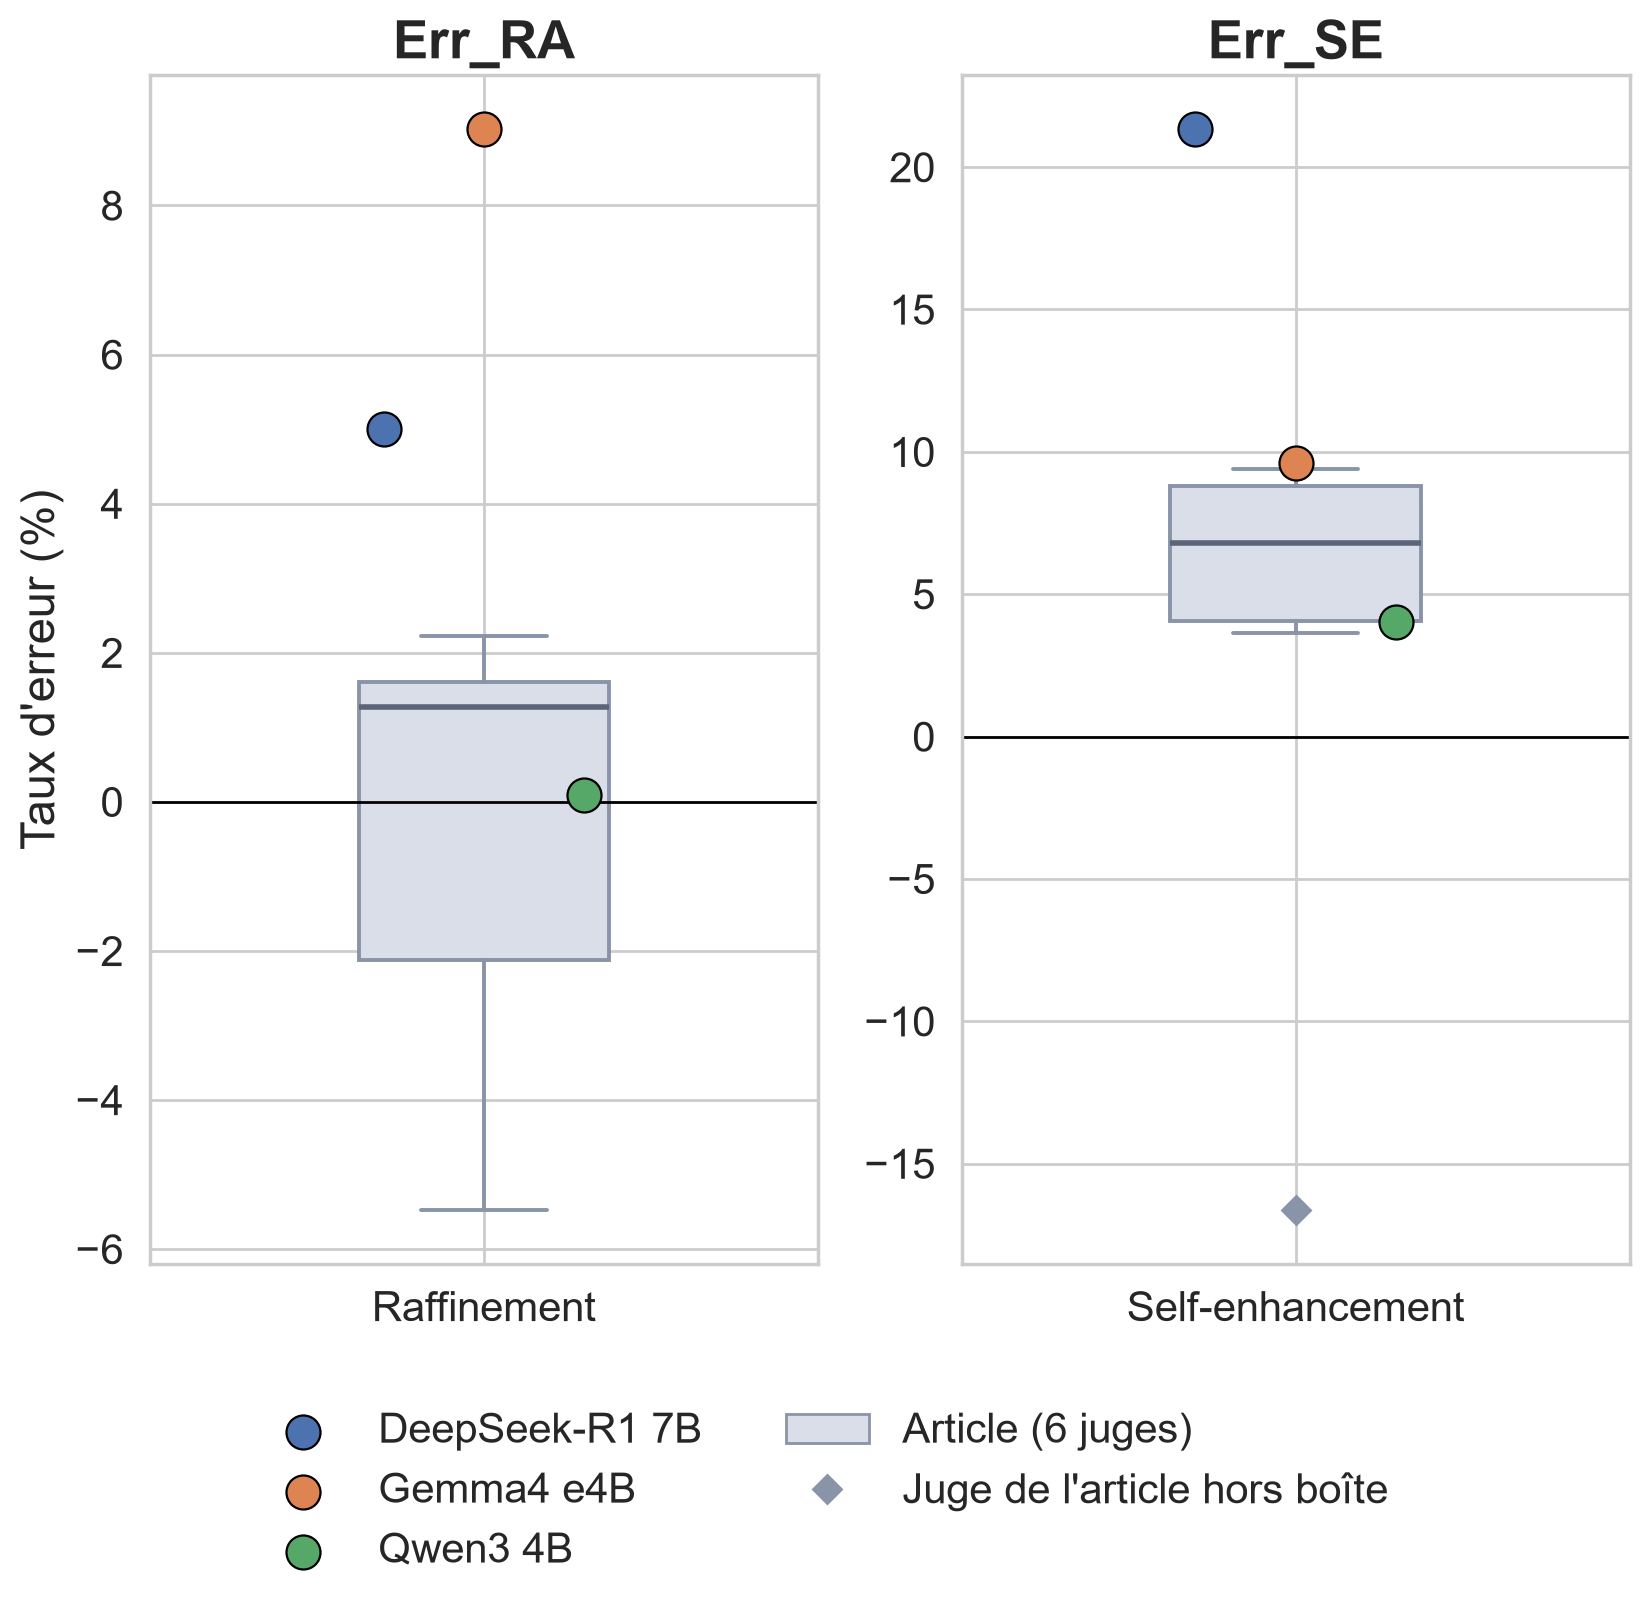
\includegraphics[width=0.88\textwidth]{figures/notation.png}
  \caption{Erreurs de raffinement ($\ErrRA$) et d'auto-valorisation ($\ErrSE$), en pourcents. Une erreur proche de zéro est souhaitable.}
  \label{fig-notation}
\end{figure}
